\documentclass[conference]{IEEEtran}
\IEEEoverridecommandlockouts

\usepackage{cite}
\usepackage{amsmath,amssymb,amsfonts}
\usepackage{algorithmic}
\usepackage{graphicx}
\usepackage{textcomp}
\usepackage{xcolor}
\usepackage{booktabs}
\usepackage{multirow}
\usepackage{bm}
\usepackage{url}
\usepackage{amssymb}
\usepackage[caption=false,font=footnotesize]{subfig}

\graphicspath{{../results/figures/}}
% Allow several two-column figures per page so that floats stay near their text.
\setcounter{dbltopnumber}{3}
\renewcommand{\dbltopfraction}{0.92}
\renewcommand{\dblfloatpagefraction}{0.85}
\renewcommand{\topfraction}{0.9}
\renewcommand{\textfraction}{0.08}
% Every number quoted in the text is read from the generated results so that the
% manuscript always matches the experiments: \res{<model>}{<metric>}.
% Auto-generated by scripts/export_latex_tables.py -- do not edit by hand.
\makeatletter
\providecommand{\res}[2]{\@ifundefined{res@#1@#2}{\textbf{??}}{\csname res@#1@#2\endcsname}}
\expandafter\def\csname res@att_convkan_proposed@accuracy\endcsname{79.00}
\expandafter\def\csname res@att_convkan_proposed@balanced_accuracy\endcsname{67.90}
\expandafter\def\csname res@att_convkan_proposed@macro_f1\endcsname{63.05}
\expandafter\def\csname res@att_convkan_proposed@weighted_f1\endcsname{79.03}
\expandafter\def\csname res@att_convkan_proposed@macro_precision\endcsname{60.04}
\expandafter\def\csname res@att_convkan_proposed@macro_recall\endcsname{67.90}
\expandafter\def\csname res@att_convkan_proposed@macro_specificity\endcsname{95.04}
\expandafter\def\csname res@att_convkan_proposed@auroc\endcsname{94.43}
\expandafter\def\csname res@att_convkan_proposed@cohen_kappa\endcsname{0.604}
\expandafter\def\csname res@att_convkan_proposed@ece\endcsname{20.59}
\expandafter\def\csname res@att_convkan_proposed@n_test\endcsname{2005.00}
\expandafter\def\csname res@att_convkan_proposed@macro_f1_ci_lower\endcsname{59.48}
\expandafter\def\csname res@att_convkan_proposed@macro_f1_ci_upper\endcsname{66.81}
\expandafter\def\csname res@att_convkan_proposed@macro_f1_ci_std\endcsname{1.91}
\expandafter\def\csname res@att_convkan_proposed@accuracy_ci_lower\endcsname{77.21}
\expandafter\def\csname res@att_convkan_proposed@accuracy_ci_upper\endcsname{80.75}
\expandafter\def\csname res@att_convkan_proposed@accuracy_ci_std\endcsname{0.92}
\expandafter\def\csname res@att_convkan_proposed@auroc_ci_lower\endcsname{93.49}
\expandafter\def\csname res@att_convkan_proposed@auroc_ci_upper\endcsname{95.26}
\expandafter\def\csname res@att_convkan_proposed@auroc_ci_std\endcsname{0.45}
\expandafter\def\csname res@att_convkan_proposed@conformal_alpha\endcsname{0.10}
\expandafter\def\csname res@att_convkan_proposed@conformal_qhat\endcsname{0.77}
\expandafter\def\csname res@att_convkan_proposed@conformal_coverage\endcsname{89.68}
\expandafter\def\csname res@att_convkan_proposed@conformal_set_size\endcsname{1.45}
\expandafter\def\csname res@att_convkan_proposed@best_epoch\endcsname{8}
\expandafter\def\csname res@att_convkan_proposed@epochs_run\endcsname{10.00}
\expandafter\def\csname res@att_convkan_proposed@epochs_budget\endcsname{10.00}
\expandafter\def\csname res@att_convkan_proposed@train_time_min\endcsname{32.4}
\expandafter\def\csname res@att_convkan_proposed@best_val_macro_f1\endcsname{62.95}
\expandafter\def\csname res@att_convkan_proposed@image_size\endcsname{128.00}
\expandafter\def\csname res@att_convkan_proposed@spline_regularization\endcsname{1.00}
\expandafter\def\csname res@att_convkan_proposed@lambda_l1\endcsname{1.00}
\expandafter\def\csname res@att_convkan_proposed@lambda_ent\endcsname{0.10}
\expandafter\def\csname res@att_convkan_proposed@kan_head_edges\endcsname{37312.00}
\expandafter\def\csname res@att_convkan_proposed@kan_edge_sparsity\endcsname{1.000}
\expandafter\def\csname res@att_convkan_proposed@kan_spline_entropy\endcsname{0.0006}
\expandafter\def\csname res@att_convkan_proposed@kan_head_mean_l1\endcsname{4.99e-04}
\expandafter\def\csname res@att_convkan_proposed@kan_conv_mean_l1\endcsname{8.90e-04}
\expandafter\def\csname res@att_convkan_proposed@temperature\endcsname{0.528}
\expandafter\def\csname res@att_convkan_proposed@ece_temperature_scaled\endcsname{2.30}
\expandafter\def\csname res@att_convkan_proposed@kan_top_mass\endcsname{1.000}
\expandafter\def\csname res@att_convkan_proposed@post_hoc_version\endcsname{1.00}
\expandafter\def\csname res@att_convkan_proposed@params_m\endcsname{1.59}
\expandafter\def\csname res@att_convkan_proposed@params_total\endcsname{1587176.00}
\expandafter\def\csname res@att_convkan_proposed@head_params_k\endcsname{374.4}
\expandafter\def\csname res@att_convkan_proposed@head_params\endcsname{374400.00}
\expandafter\def\csname res@att_convkan_proposed@model_size_mb\endcsname{6.23}
\expandafter\def\csname res@att_convkan_proposed@gflops\endcsname{0.048}
\expandafter\def\csname res@att_convkan_proposed@gmacs\endcsname{0.02}
\expandafter\def\csname res@att_convkan_proposed@kan_basis_mflops\endcsname{4.02}
\expandafter\def\csname res@att_convkan_proposed@latency_ms\endcsname{16.09}
\expandafter\def\csname res@att_convkan_proposed@latency_std_ms\endcsname{2.44}
\expandafter\def\csname res@att_convkan_proposed@latency_median_ms\endcsname{15.51}
\expandafter\def\csname res@att_convkan_proposed@throughput_img_s\endcsname{165}
\expandafter\def\csname res@att_convkan_proposed@num_threads\endcsname{4.00}
\expandafter\def\csname res@att_convkan_proposed@checkpoint_file_mb\endcsname{6.24}
\expandafter\def\csname res@resnet50@accuracy\endcsname{82.24}
\expandafter\def\csname res@resnet50@balanced_accuracy\endcsname{75.00}
\expandafter\def\csname res@resnet50@macro_f1\endcsname{71.96}
\expandafter\def\csname res@resnet50@weighted_f1\endcsname{82.03}
\expandafter\def\csname res@resnet50@macro_precision\endcsname{69.75}
\expandafter\def\csname res@resnet50@macro_recall\endcsname{75.00}
\expandafter\def\csname res@resnet50@macro_specificity\endcsname{95.67}
\expandafter\def\csname res@resnet50@auroc\endcsname{95.63}
\expandafter\def\csname res@resnet50@cohen_kappa\endcsname{0.663}
\expandafter\def\csname res@resnet50@ece\endcsname{18.96}
\expandafter\def\csname res@resnet50@n_test\endcsname{2005.00}
\expandafter\def\csname res@resnet50@macro_f1_ci_lower\endcsname{68.37}
\expandafter\def\csname res@resnet50@macro_f1_ci_upper\endcsname{75.21}
\expandafter\def\csname res@resnet50@macro_f1_ci_std\endcsname{1.74}
\expandafter\def\csname res@resnet50@accuracy_ci_lower\endcsname{80.65}
\expandafter\def\csname res@resnet50@accuracy_ci_upper\endcsname{83.89}
\expandafter\def\csname res@resnet50@accuracy_ci_std\endcsname{0.85}
\expandafter\def\csname res@resnet50@auroc_ci_lower\endcsname{94.55}
\expandafter\def\csname res@resnet50@auroc_ci_upper\endcsname{96.62}
\expandafter\def\csname res@resnet50@auroc_ci_std\endcsname{0.54}
\expandafter\def\csname res@resnet50@conformal_alpha\endcsname{0.10}
\expandafter\def\csname res@resnet50@conformal_qhat\endcsname{0.74}
\expandafter\def\csname res@resnet50@conformal_coverage\endcsname{90.97}
\expandafter\def\csname res@resnet50@conformal_set_size\endcsname{1.29}
\expandafter\def\csname res@resnet50@best_epoch\endcsname{9}
\expandafter\def\csname res@resnet50@epochs_run\endcsname{10.00}
\expandafter\def\csname res@resnet50@epochs_budget\endcsname{10.00}
\expandafter\def\csname res@resnet50@train_time_min\endcsname{81.8}
\expandafter\def\csname res@resnet50@best_val_macro_f1\endcsname{71.84}
\expandafter\def\csname res@resnet50@image_size\endcsname{128.00}
\expandafter\def\csname res@resnet50@spline_regularization\endcsname{0.00}
\expandafter\def\csname res@resnet50@lambda_l1\endcsname{0.00}
\expandafter\def\csname res@resnet50@lambda_ent\endcsname{0.00}
\expandafter\def\csname res@resnet50@temperature\endcsname{0.521}
\expandafter\def\csname res@resnet50@ece_temperature_scaled\endcsname{2.43}
\expandafter\def\csname res@resnet50@post_hoc_version\endcsname{1.00}
\expandafter\def\csname res@resnet50@params_m\endcsname{23.52}
\expandafter\def\csname res@resnet50@params_total\endcsname{23522375.00}
\expandafter\def\csname res@resnet50@head_params_k\endcsname{14.3}
\expandafter\def\csname res@resnet50@head_params\endcsname{14343.00}
\expandafter\def\csname res@resnet50@model_size_mb\endcsname{90.03}
\expandafter\def\csname res@resnet50@gflops\endcsname{2.669}
\expandafter\def\csname res@resnet50@gmacs\endcsname{1.33}
\expandafter\def\csname res@resnet50@kan_basis_mflops\endcsname{0.00}
\expandafter\def\csname res@resnet50@latency_ms\endcsname{48.00}
\expandafter\def\csname res@resnet50@latency_std_ms\endcsname{8.75}
\expandafter\def\csname res@resnet50@latency_median_ms\endcsname{46.11}
\expandafter\def\csname res@resnet50@throughput_img_s\endcsname{44}
\expandafter\def\csname res@resnet50@num_threads\endcsname{4.00}
\expandafter\def\csname res@resnet50@checkpoint_file_mb\endcsname{90.03}
\expandafter\def\csname res@densenet121@accuracy\endcsname{84.54}
\expandafter\def\csname res@densenet121@balanced_accuracy\endcsname{76.31}
\expandafter\def\csname res@densenet121@macro_f1\endcsname{75.16}
\expandafter\def\csname res@densenet121@weighted_f1\endcsname{84.80}
\expandafter\def\csname res@densenet121@macro_precision\endcsname{74.10}
\expandafter\def\csname res@densenet121@macro_recall\endcsname{76.31}
\expandafter\def\csname res@densenet121@macro_specificity\endcsname{96.52}
\expandafter\def\csname res@densenet121@auroc\endcsname{96.80}
\expandafter\def\csname res@densenet121@cohen_kappa\endcsname{0.712}
\expandafter\def\csname res@densenet121@ece\endcsname{17.70}
\expandafter\def\csname res@densenet121@n_test\endcsname{2005.00}
\expandafter\def\csname res@densenet121@macro_f1_ci_lower\endcsname{71.45}
\expandafter\def\csname res@densenet121@macro_f1_ci_upper\endcsname{78.51}
\expandafter\def\csname res@densenet121@macro_f1_ci_std\endcsname{1.80}
\expandafter\def\csname res@densenet121@accuracy_ci_lower\endcsname{82.94}
\expandafter\def\csname res@densenet121@accuracy_ci_upper\endcsname{86.08}
\expandafter\def\csname res@densenet121@accuracy_ci_std\endcsname{0.81}
\expandafter\def\csname res@densenet121@auroc_ci_lower\endcsname{96.04}
\expandafter\def\csname res@densenet121@auroc_ci_upper\endcsname{97.41}
\expandafter\def\csname res@densenet121@auroc_ci_std\endcsname{0.35}
\expandafter\def\csname res@densenet121@conformal_alpha\endcsname{0.10}
\expandafter\def\csname res@densenet121@conformal_qhat\endcsname{0.70}
\expandafter\def\csname res@densenet121@conformal_coverage\endcsname{90.12}
\expandafter\def\csname res@densenet121@conformal_set_size\endcsname{1.17}
\expandafter\def\csname res@densenet121@best_epoch\endcsname{9}
\expandafter\def\csname res@densenet121@epochs_run\endcsname{10.00}
\expandafter\def\csname res@densenet121@epochs_budget\endcsname{10.00}
\expandafter\def\csname res@densenet121@train_time_min\endcsname{70.0}
\expandafter\def\csname res@densenet121@best_val_macro_f1\endcsname{75.09}
\expandafter\def\csname res@densenet121@image_size\endcsname{128.00}
\expandafter\def\csname res@densenet121@spline_regularization\endcsname{0.00}
\expandafter\def\csname res@densenet121@lambda_l1\endcsname{0.00}
\expandafter\def\csname res@densenet121@lambda_ent\endcsname{0.00}
\expandafter\def\csname res@densenet121@temperature\endcsname{0.538}
\expandafter\def\csname res@densenet121@ece_temperature_scaled\endcsname{1.86}
\expandafter\def\csname res@densenet121@post_hoc_version\endcsname{1.00}
\expandafter\def\csname res@densenet121@params_m\endcsname{6.96}
\expandafter\def\csname res@densenet121@params_total\endcsname{6961031.00}
\expandafter\def\csname res@densenet121@head_params_k\endcsname{7.2}
\expandafter\def\csname res@densenet121@head_params\endcsname{7175.00}
\expandafter\def\csname res@densenet121@model_size_mb\endcsname{27.13}
\expandafter\def\csname res@densenet121@gflops\endcsname{1.850}
\expandafter\def\csname res@densenet121@gmacs\endcsname{0.93}
\expandafter\def\csname res@densenet121@kan_basis_mflops\endcsname{0.00}
\expandafter\def\csname res@densenet121@latency_ms\endcsname{62.98}
\expandafter\def\csname res@densenet121@latency_std_ms\endcsname{7.98}
\expandafter\def\csname res@densenet121@latency_median_ms\endcsname{63.69}
\expandafter\def\csname res@densenet121@throughput_img_s\endcsname{45}
\expandafter\def\csname res@densenet121@num_threads\endcsname{4.00}
\expandafter\def\csname res@densenet121@checkpoint_file_mb\endcsname{27.14}
\expandafter\def\csname res@mobilenetv3_small@accuracy\endcsname{77.46}
\expandafter\def\csname res@mobilenetv3_small@balanced_accuracy\endcsname{67.70}
\expandafter\def\csname res@mobilenetv3_small@macro_f1\endcsname{62.27}
\expandafter\def\csname res@mobilenetv3_small@weighted_f1\endcsname{77.74}
\expandafter\def\csname res@mobilenetv3_small@macro_precision\endcsname{58.79}
\expandafter\def\csname res@mobilenetv3_small@macro_recall\endcsname{67.70}
\expandafter\def\csname res@mobilenetv3_small@macro_specificity\endcsname{94.91}
\expandafter\def\csname res@mobilenetv3_small@auroc\endcsname{94.05}
\expandafter\def\csname res@mobilenetv3_small@cohen_kappa\endcsname{0.582}
\expandafter\def\csname res@mobilenetv3_small@ece\endcsname{18.19}
\expandafter\def\csname res@mobilenetv3_small@n_test\endcsname{2005.00}
\expandafter\def\csname res@mobilenetv3_small@macro_f1_ci_lower\endcsname{58.55}
\expandafter\def\csname res@mobilenetv3_small@macro_f1_ci_upper\endcsname{65.64}
\expandafter\def\csname res@mobilenetv3_small@macro_f1_ci_std\endcsname{1.88}
\expandafter\def\csname res@mobilenetv3_small@accuracy_ci_lower\endcsname{75.66}
\expandafter\def\csname res@mobilenetv3_small@accuracy_ci_upper\endcsname{79.30}
\expandafter\def\csname res@mobilenetv3_small@accuracy_ci_std\endcsname{0.94}
\expandafter\def\csname res@mobilenetv3_small@auroc_ci_lower\endcsname{93.20}
\expandafter\def\csname res@mobilenetv3_small@auroc_ci_upper\endcsname{94.78}
\expandafter\def\csname res@mobilenetv3_small@auroc_ci_std\endcsname{0.39}
\expandafter\def\csname res@mobilenetv3_small@conformal_alpha\endcsname{0.10}
\expandafter\def\csname res@mobilenetv3_small@conformal_qhat\endcsname{0.77}
\expandafter\def\csname res@mobilenetv3_small@conformal_coverage\endcsname{89.68}
\expandafter\def\csname res@mobilenetv3_small@conformal_set_size\endcsname{1.49}
\expandafter\def\csname res@mobilenetv3_small@best_epoch\endcsname{10}
\expandafter\def\csname res@mobilenetv3_small@epochs_run\endcsname{10.00}
\expandafter\def\csname res@mobilenetv3_small@epochs_budget\endcsname{10.00}
\expandafter\def\csname res@mobilenetv3_small@train_time_min\endcsname{13.1}
\expandafter\def\csname res@mobilenetv3_small@best_val_macro_f1\endcsname{65.01}
\expandafter\def\csname res@mobilenetv3_small@image_size\endcsname{128.00}
\expandafter\def\csname res@mobilenetv3_small@spline_regularization\endcsname{0.00}
\expandafter\def\csname res@mobilenetv3_small@lambda_l1\endcsname{0.00}
\expandafter\def\csname res@mobilenetv3_small@lambda_ent\endcsname{0.00}
\expandafter\def\csname res@mobilenetv3_small@temperature\endcsname{0.534}
\expandafter\def\csname res@mobilenetv3_small@ece_temperature_scaled\endcsname{2.69}
\expandafter\def\csname res@mobilenetv3_small@post_hoc_version\endcsname{1.00}
\expandafter\def\csname res@mobilenetv3_small@params_m\endcsname{1.53}
\expandafter\def\csname res@mobilenetv3_small@params_total\endcsname{1525031.00}
\expandafter\def\csname res@mobilenetv3_small@head_params_k\endcsname{598.0}
\expandafter\def\csname res@mobilenetv3_small@head_params\endcsname{598023.00}
\expandafter\def\csname res@mobilenetv3_small@model_size_mb\endcsname{5.94}
\expandafter\def\csname res@mobilenetv3_small@gflops\endcsname{0.038}
\expandafter\def\csname res@mobilenetv3_small@gmacs\endcsname{0.02}
\expandafter\def\csname res@mobilenetv3_small@kan_basis_mflops\endcsname{0.00}
\expandafter\def\csname res@mobilenetv3_small@latency_ms\endcsname{9.00}
\expandafter\def\csname res@mobilenetv3_small@latency_std_ms\endcsname{1.69}
\expandafter\def\csname res@mobilenetv3_small@latency_median_ms\endcsname{8.56}
\expandafter\def\csname res@mobilenetv3_small@throughput_img_s\endcsname{582}
\expandafter\def\csname res@mobilenetv3_small@num_threads\endcsname{4.00}
\expandafter\def\csname res@mobilenetv3_small@checkpoint_file_mb\endcsname{5.95}
\expandafter\def\csname res@vit_tiny@accuracy\endcsname{83.09}
\expandafter\def\csname res@vit_tiny@balanced_accuracy\endcsname{79.27}
\expandafter\def\csname res@vit_tiny@macro_f1\endcsname{74.43}
\expandafter\def\csname res@vit_tiny@weighted_f1\endcsname{83.31}
\expandafter\def\csname res@vit_tiny@macro_precision\endcsname{70.82}
\expandafter\def\csname res@vit_tiny@macro_recall\endcsname{79.27}
\expandafter\def\csname res@vit_tiny@macro_specificity\endcsname{96.12}
\expandafter\def\csname res@vit_tiny@auroc\endcsname{96.55}
\expandafter\def\csname res@vit_tiny@cohen_kappa\endcsname{0.685}
\expandafter\def\csname res@vit_tiny@ece\endcsname{21.31}
\expandafter\def\csname res@vit_tiny@n_test\endcsname{2005.00}
\expandafter\def\csname res@vit_tiny@macro_f1_ci_lower\endcsname{71.08}
\expandafter\def\csname res@vit_tiny@macro_f1_ci_upper\endcsname{77.50}
\expandafter\def\csname res@vit_tiny@macro_f1_ci_std\endcsname{1.65}
\expandafter\def\csname res@vit_tiny@accuracy_ci_lower\endcsname{81.40}
\expandafter\def\csname res@vit_tiny@accuracy_ci_upper\endcsname{84.74}
\expandafter\def\csname res@vit_tiny@accuracy_ci_std\endcsname{0.84}
\expandafter\def\csname res@vit_tiny@auroc_ci_lower\endcsname{96.06}
\expandafter\def\csname res@vit_tiny@auroc_ci_upper\endcsname{97.02}
\expandafter\def\csname res@vit_tiny@auroc_ci_std\endcsname{0.25}
\expandafter\def\csname res@vit_tiny@conformal_alpha\endcsname{0.10}
\expandafter\def\csname res@vit_tiny@conformal_qhat\endcsname{0.72}
\expandafter\def\csname res@vit_tiny@conformal_coverage\endcsname{90.67}
\expandafter\def\csname res@vit_tiny@conformal_set_size\endcsname{1.28}
\expandafter\def\csname res@vit_tiny@best_epoch\endcsname{9}
\expandafter\def\csname res@vit_tiny@epochs_run\endcsname{10.00}
\expandafter\def\csname res@vit_tiny@epochs_budget\endcsname{10.00}
\expandafter\def\csname res@vit_tiny@train_time_min\endcsname{26.6}
\expandafter\def\csname res@vit_tiny@best_val_macro_f1\endcsname{71.15}
\expandafter\def\csname res@vit_tiny@image_size\endcsname{128.00}
\expandafter\def\csname res@vit_tiny@spline_regularization\endcsname{0.00}
\expandafter\def\csname res@vit_tiny@lambda_l1\endcsname{0.00}
\expandafter\def\csname res@vit_tiny@lambda_ent\endcsname{0.00}
\expandafter\def\csname res@vit_tiny@temperature\endcsname{0.494}
\expandafter\def\csname res@vit_tiny@ece_temperature_scaled\endcsname{1.56}
\expandafter\def\csname res@vit_tiny@post_hoc_version\endcsname{1.00}
\expandafter\def\csname res@vit_tiny@params_m\endcsname{5.50}
\expandafter\def\csname res@vit_tiny@params_total\endcsname{5500423.00}
\expandafter\def\csname res@vit_tiny@head_params_k\endcsname{1.4}
\expandafter\def\csname res@vit_tiny@head_params\endcsname{1351.00}
\expandafter\def\csname res@vit_tiny@model_size_mb\endcsname{21.04}
\expandafter\def\csname res@vit_tiny@gflops\endcsname{0.709}
\expandafter\def\csname res@vit_tiny@gmacs\endcsname{0.35}
\expandafter\def\csname res@vit_tiny@kan_basis_mflops\endcsname{0.00}
\expandafter\def\csname res@vit_tiny@latency_ms\endcsname{14.77}
\expandafter\def\csname res@vit_tiny@latency_std_ms\endcsname{2.90}
\expandafter\def\csname res@vit_tiny@latency_median_ms\endcsname{14.17}
\expandafter\def\csname res@vit_tiny@throughput_img_s\endcsname{211}
\expandafter\def\csname res@vit_tiny@num_threads\endcsname{4.00}
\expandafter\def\csname res@vit_tiny@checkpoint_file_mb\endcsname{21.04}
\expandafter\def\csname res@convnext_tiny@accuracy\endcsname{82.49}
\expandafter\def\csname res@convnext_tiny@balanced_accuracy\endcsname{76.16}
\expandafter\def\csname res@convnext_tiny@macro_f1\endcsname{72.35}
\expandafter\def\csname res@convnext_tiny@weighted_f1\endcsname{82.58}
\expandafter\def\csname res@convnext_tiny@macro_precision\endcsname{69.40}
\expandafter\def\csname res@convnext_tiny@macro_recall\endcsname{76.16}
\expandafter\def\csname res@convnext_tiny@macro_specificity\endcsname{95.88}
\expandafter\def\csname res@convnext_tiny@auroc\endcsname{96.41}
\expandafter\def\csname res@convnext_tiny@cohen_kappa\endcsname{0.673}
\expandafter\def\csname res@convnext_tiny@ece\endcsname{20.35}
\expandafter\def\csname res@convnext_tiny@n_test\endcsname{2005.00}
\expandafter\def\csname res@convnext_tiny@macro_f1_ci_lower\endcsname{68.57}
\expandafter\def\csname res@convnext_tiny@macro_f1_ci_upper\endcsname{75.63}
\expandafter\def\csname res@convnext_tiny@macro_f1_ci_std\endcsname{1.79}
\expandafter\def\csname res@convnext_tiny@accuracy_ci_lower\endcsname{80.70}
\expandafter\def\csname res@convnext_tiny@accuracy_ci_upper\endcsname{84.19}
\expandafter\def\csname res@convnext_tiny@accuracy_ci_std\endcsname{0.86}
\expandafter\def\csname res@convnext_tiny@auroc_ci_lower\endcsname{95.73}
\expandafter\def\csname res@convnext_tiny@auroc_ci_upper\endcsname{96.96}
\expandafter\def\csname res@convnext_tiny@auroc_ci_std\endcsname{0.31}
\expandafter\def\csname res@convnext_tiny@conformal_alpha\endcsname{0.10}
\expandafter\def\csname res@convnext_tiny@conformal_qhat\endcsname{0.73}
\expandafter\def\csname res@convnext_tiny@conformal_coverage\endcsname{91.22}
\expandafter\def\csname res@convnext_tiny@conformal_set_size\endcsname{1.28}
\expandafter\def\csname res@convnext_tiny@best_epoch\endcsname{10}
\expandafter\def\csname res@convnext_tiny@epochs_run\endcsname{10.00}
\expandafter\def\csname res@convnext_tiny@epochs_budget\endcsname{10.00}
\expandafter\def\csname res@convnext_tiny@train_time_min\endcsname{82.4}
\expandafter\def\csname res@convnext_tiny@best_val_macro_f1\endcsname{70.23}
\expandafter\def\csname res@convnext_tiny@image_size\endcsname{128.00}
\expandafter\def\csname res@convnext_tiny@spline_regularization\endcsname{0.00}
\expandafter\def\csname res@convnext_tiny@lambda_l1\endcsname{0.00}
\expandafter\def\csname res@convnext_tiny@lambda_ent\endcsname{0.00}
\expandafter\def\csname res@convnext_tiny@temperature\endcsname{0.512}
\expandafter\def\csname res@convnext_tiny@ece_temperature_scaled\endcsname{2.77}
\expandafter\def\csname res@convnext_tiny@post_hoc_version\endcsname{1.00}
\expandafter\def\csname res@convnext_tiny@params_m\endcsname{27.83}
\expandafter\def\csname res@convnext_tiny@params_total\endcsname{27825511.00}
\expandafter\def\csname res@convnext_tiny@head_params_k\endcsname{6.9}
\expandafter\def\csname res@convnext_tiny@head_params\endcsname{6919.00}
\expandafter\def\csname res@convnext_tiny@model_size_mb\endcsname{106.21}
\expandafter\def\csname res@convnext_tiny@gflops\endcsname{2.909}
\expandafter\def\csname res@convnext_tiny@gmacs\endcsname{1.45}
\expandafter\def\csname res@convnext_tiny@kan_basis_mflops\endcsname{0.00}
\expandafter\def\csname res@convnext_tiny@latency_ms\endcsname{52.11}
\expandafter\def\csname res@convnext_tiny@latency_std_ms\endcsname{6.51}
\expandafter\def\csname res@convnext_tiny@latency_median_ms\endcsname{53.51}
\expandafter\def\csname res@convnext_tiny@throughput_img_s\endcsname{53}
\expandafter\def\csname res@convnext_tiny@num_threads\endcsname{4.00}
\expandafter\def\csname res@convnext_tiny@checkpoint_file_mb\endcsname{106.21}
\expandafter\def\csname res@ablation_1_backbone_mlp@accuracy\endcsname{79.30}
\expandafter\def\csname res@ablation_1_backbone_mlp@balanced_accuracy\endcsname{69.07}
\expandafter\def\csname res@ablation_1_backbone_mlp@macro_f1\endcsname{64.67}
\expandafter\def\csname res@ablation_1_backbone_mlp@weighted_f1\endcsname{78.97}
\expandafter\def\csname res@ablation_1_backbone_mlp@macro_precision\endcsname{62.17}
\expandafter\def\csname res@ablation_1_backbone_mlp@macro_recall\endcsname{69.07}
\expandafter\def\csname res@ablation_1_backbone_mlp@macro_specificity\endcsname{94.88}
\expandafter\def\csname res@ablation_1_backbone_mlp@auroc\endcsname{94.65}
\expandafter\def\csname res@ablation_1_backbone_mlp@cohen_kappa\endcsname{0.604}
\expandafter\def\csname res@ablation_1_backbone_mlp@ece\endcsname{20.50}
\expandafter\def\csname res@ablation_1_backbone_mlp@n_test\endcsname{2005.00}
\expandafter\def\csname res@ablation_1_backbone_mlp@macro_f1_ci_lower\endcsname{60.72}
\expandafter\def\csname res@ablation_1_backbone_mlp@macro_f1_ci_upper\endcsname{68.26}
\expandafter\def\csname res@ablation_1_backbone_mlp@macro_f1_ci_std\endcsname{1.89}
\expandafter\def\csname res@ablation_1_backbone_mlp@accuracy_ci_lower\endcsname{77.55}
\expandafter\def\csname res@ablation_1_backbone_mlp@accuracy_ci_upper\endcsname{81.15}
\expandafter\def\csname res@ablation_1_backbone_mlp@accuracy_ci_std\endcsname{0.91}
\expandafter\def\csname res@ablation_1_backbone_mlp@auroc_ci_lower\endcsname{93.89}
\expandafter\def\csname res@ablation_1_backbone_mlp@auroc_ci_upper\endcsname{95.36}
\expandafter\def\csname res@ablation_1_backbone_mlp@auroc_ci_std\endcsname{0.38}
\expandafter\def\csname res@ablation_1_backbone_mlp@conformal_alpha\endcsname{0.10}
\expandafter\def\csname res@ablation_1_backbone_mlp@conformal_qhat\endcsname{0.75}
\expandafter\def\csname res@ablation_1_backbone_mlp@conformal_coverage\endcsname{90.77}
\expandafter\def\csname res@ablation_1_backbone_mlp@conformal_set_size\endcsname{1.45}
\expandafter\def\csname res@ablation_1_backbone_mlp@best_epoch\endcsname{9}
\expandafter\def\csname res@ablation_1_backbone_mlp@epochs_run\endcsname{10.00}
\expandafter\def\csname res@ablation_1_backbone_mlp@epochs_budget\endcsname{10.00}
\expandafter\def\csname res@ablation_1_backbone_mlp@train_time_min\endcsname{11.1}
\expandafter\def\csname res@ablation_1_backbone_mlp@best_val_macro_f1\endcsname{66.60}
\expandafter\def\csname res@ablation_1_backbone_mlp@image_size\endcsname{128.00}
\expandafter\def\csname res@ablation_1_backbone_mlp@spline_regularization\endcsname{0.00}
\expandafter\def\csname res@ablation_1_backbone_mlp@lambda_l1\endcsname{0.00}
\expandafter\def\csname res@ablation_1_backbone_mlp@lambda_ent\endcsname{0.00}
\expandafter\def\csname res@ablation_1_backbone_mlp@temperature\endcsname{0.507}
\expandafter\def\csname res@ablation_1_backbone_mlp@ece_temperature_scaled\endcsname{2.45}
\expandafter\def\csname res@ablation_1_backbone_mlp@post_hoc_version\endcsname{1.00}
\expandafter\def\csname res@ablation_1_backbone_mlp@params_m\endcsname{1.53}
\expandafter\def\csname res@ablation_1_backbone_mlp@params_total\endcsname{1526183.00}
\expandafter\def\csname res@ablation_1_backbone_mlp@head_params_k\endcsname{599.2}
\expandafter\def\csname res@ablation_1_backbone_mlp@head_params\endcsname{599175.00}
\expandafter\def\csname res@ablation_1_backbone_mlp@model_size_mb\endcsname{5.95}
\expandafter\def\csname res@ablation_1_backbone_mlp@gflops\endcsname{0.038}
\expandafter\def\csname res@ablation_1_backbone_mlp@gmacs\endcsname{0.02}
\expandafter\def\csname res@ablation_1_backbone_mlp@kan_basis_mflops\endcsname{0.00}
\expandafter\def\csname res@ablation_1_backbone_mlp@latency_ms\endcsname{10.52}
\expandafter\def\csname res@ablation_1_backbone_mlp@latency_std_ms\endcsname{3.02}
\expandafter\def\csname res@ablation_1_backbone_mlp@latency_median_ms\endcsname{9.50}
\expandafter\def\csname res@ablation_1_backbone_mlp@throughput_img_s\endcsname{600}
\expandafter\def\csname res@ablation_1_backbone_mlp@num_threads\endcsname{4.00}
\expandafter\def\csname res@ablation_1_backbone_mlp@checkpoint_file_mb\endcsname{5.96}
\expandafter\def\csname res@ablation_2_backbone_kan_no_att@accuracy\endcsname{79.15}
\expandafter\def\csname res@ablation_2_backbone_kan_no_att@balanced_accuracy\endcsname{70.12}
\expandafter\def\csname res@ablation_2_backbone_kan_no_att@macro_f1\endcsname{65.57}
\expandafter\def\csname res@ablation_2_backbone_kan_no_att@weighted_f1\endcsname{79.65}
\expandafter\def\csname res@ablation_2_backbone_kan_no_att@macro_precision\endcsname{62.10}
\expandafter\def\csname res@ablation_2_backbone_kan_no_att@macro_recall\endcsname{70.12}
\expandafter\def\csname res@ablation_2_backbone_kan_no_att@macro_specificity\endcsname{95.42}
\expandafter\def\csname res@ablation_2_backbone_kan_no_att@auroc\endcsname{95.19}
\expandafter\def\csname res@ablation_2_backbone_kan_no_att@cohen_kappa\endcsname{0.617}
\expandafter\def\csname res@ablation_2_backbone_kan_no_att@ece\endcsname{20.00}
\expandafter\def\csname res@ablation_2_backbone_kan_no_att@n_test\endcsname{2005.00}
\expandafter\def\csname res@ablation_2_backbone_kan_no_att@macro_f1_ci_lower\endcsname{61.64}
\expandafter\def\csname res@ablation_2_backbone_kan_no_att@macro_f1_ci_upper\endcsname{69.12}
\expandafter\def\csname res@ablation_2_backbone_kan_no_att@macro_f1_ci_std\endcsname{1.90}
\expandafter\def\csname res@ablation_2_backbone_kan_no_att@accuracy_ci_lower\endcsname{77.26}
\expandafter\def\csname res@ablation_2_backbone_kan_no_att@accuracy_ci_upper\endcsname{81.00}
\expandafter\def\csname res@ablation_2_backbone_kan_no_att@accuracy_ci_std\endcsname{0.93}
\expandafter\def\csname res@ablation_2_backbone_kan_no_att@auroc_ci_lower\endcsname{94.40}
\expandafter\def\csname res@ablation_2_backbone_kan_no_att@auroc_ci_upper\endcsname{95.88}
\expandafter\def\csname res@ablation_2_backbone_kan_no_att@auroc_ci_std\endcsname{0.38}
\expandafter\def\csname res@ablation_2_backbone_kan_no_att@conformal_alpha\endcsname{0.10}
\expandafter\def\csname res@ablation_2_backbone_kan_no_att@conformal_qhat\endcsname{0.76}
\expandafter\def\csname res@ablation_2_backbone_kan_no_att@conformal_coverage\endcsname{90.92}
\expandafter\def\csname res@ablation_2_backbone_kan_no_att@conformal_set_size\endcsname{1.44}
\expandafter\def\csname res@ablation_2_backbone_kan_no_att@best_epoch\endcsname{9}
\expandafter\def\csname res@ablation_2_backbone_kan_no_att@epochs_run\endcsname{10.00}
\expandafter\def\csname res@ablation_2_backbone_kan_no_att@epochs_budget\endcsname{10.00}
\expandafter\def\csname res@ablation_2_backbone_kan_no_att@train_time_min\endcsname{10.5}
\expandafter\def\csname res@ablation_2_backbone_kan_no_att@best_val_macro_f1\endcsname{64.98}
\expandafter\def\csname res@ablation_2_backbone_kan_no_att@image_size\endcsname{128.00}
\expandafter\def\csname res@ablation_2_backbone_kan_no_att@spline_regularization\endcsname{1.00}
\expandafter\def\csname res@ablation_2_backbone_kan_no_att@lambda_l1\endcsname{1.00}
\expandafter\def\csname res@ablation_2_backbone_kan_no_att@lambda_ent\endcsname{0.10}
\expandafter\def\csname res@ablation_2_backbone_kan_no_att@kan_head_edges\endcsname{37312.00}
\expandafter\def\csname res@ablation_2_backbone_kan_no_att@kan_edge_sparsity\endcsname{1.000}
\expandafter\def\csname res@ablation_2_backbone_kan_no_att@kan_spline_entropy\endcsname{0.0610}
\expandafter\def\csname res@ablation_2_backbone_kan_no_att@kan_head_mean_l1\endcsname{5.14e-04}
\expandafter\def\csname res@ablation_2_backbone_kan_no_att@kan_conv_mean_l1\endcsname{0.00e+00}
\expandafter\def\csname res@ablation_2_backbone_kan_no_att@temperature\endcsname{0.545}
\expandafter\def\csname res@ablation_2_backbone_kan_no_att@ece_temperature_scaled\endcsname{3.84}
\expandafter\def\csname res@ablation_2_backbone_kan_no_att@kan_top_mass\endcsname{1.000}
\expandafter\def\csname res@ablation_2_backbone_kan_no_att@post_hoc_version\endcsname{1.00}
\expandafter\def\csname res@ablation_2_backbone_kan_no_att@params_m\endcsname{1.30}
\expandafter\def\csname res@ablation_2_backbone_kan_no_att@params_total\endcsname{1301408.00}
\expandafter\def\csname res@ablation_2_backbone_kan_no_att@head_params_k\endcsname{374.4}
\expandafter\def\csname res@ablation_2_backbone_kan_no_att@head_params\endcsname{374400.00}
\expandafter\def\csname res@ablation_2_backbone_kan_no_att@model_size_mb\endcsname{5.12}
\expandafter\def\csname res@ablation_2_backbone_kan_no_att@gflops\endcsname{0.037}
\expandafter\def\csname res@ablation_2_backbone_kan_no_att@gmacs\endcsname{0.02}
\expandafter\def\csname res@ablation_2_backbone_kan_no_att@kan_basis_mflops\endcsname{0.12}
\expandafter\def\csname res@ablation_2_backbone_kan_no_att@latency_ms\endcsname{11.16}
\expandafter\def\csname res@ablation_2_backbone_kan_no_att@latency_std_ms\endcsname{2.30}
\expandafter\def\csname res@ablation_2_backbone_kan_no_att@latency_median_ms\endcsname{10.14}
\expandafter\def\csname res@ablation_2_backbone_kan_no_att@throughput_img_s\endcsname{595}
\expandafter\def\csname res@ablation_2_backbone_kan_no_att@num_threads\endcsname{4.00}
\expandafter\def\csname res@ablation_2_backbone_kan_no_att@checkpoint_file_mb\endcsname{5.13}
\expandafter\def\csname res@ablation_3_backbone_att_mlp@accuracy\endcsname{78.15}
\expandafter\def\csname res@ablation_3_backbone_att_mlp@balanced_accuracy\endcsname{70.90}
\expandafter\def\csname res@ablation_3_backbone_att_mlp@macro_f1\endcsname{62.87}
\expandafter\def\csname res@ablation_3_backbone_att_mlp@weighted_f1\endcsname{78.16}
\expandafter\def\csname res@ablation_3_backbone_att_mlp@macro_precision\endcsname{59.64}
\expandafter\def\csname res@ablation_3_backbone_att_mlp@macro_recall\endcsname{70.90}
\expandafter\def\csname res@ablation_3_backbone_att_mlp@macro_specificity\endcsname{94.88}
\expandafter\def\csname res@ablation_3_backbone_att_mlp@auroc\endcsname{94.73}
\expandafter\def\csname res@ablation_3_backbone_att_mlp@cohen_kappa\endcsname{0.590}
\expandafter\def\csname res@ablation_3_backbone_att_mlp@ece\endcsname{17.73}
\expandafter\def\csname res@ablation_3_backbone_att_mlp@n_test\endcsname{2005.00}
\expandafter\def\csname res@ablation_3_backbone_att_mlp@macro_f1_ci_lower\endcsname{59.49}
\expandafter\def\csname res@ablation_3_backbone_att_mlp@macro_f1_ci_upper\endcsname{66.07}
\expandafter\def\csname res@ablation_3_backbone_att_mlp@macro_f1_ci_std\endcsname{1.77}
\expandafter\def\csname res@ablation_3_backbone_att_mlp@accuracy_ci_lower\endcsname{76.41}
\expandafter\def\csname res@ablation_3_backbone_att_mlp@accuracy_ci_upper\endcsname{79.95}
\expandafter\def\csname res@ablation_3_backbone_att_mlp@accuracy_ci_std\endcsname{0.93}
\expandafter\def\csname res@ablation_3_backbone_att_mlp@auroc_ci_lower\endcsname{94.13}
\expandafter\def\csname res@ablation_3_backbone_att_mlp@auroc_ci_upper\endcsname{95.33}
\expandafter\def\csname res@ablation_3_backbone_att_mlp@auroc_ci_std\endcsname{0.31}
\expandafter\def\csname res@ablation_3_backbone_att_mlp@conformal_alpha\endcsname{0.10}
\expandafter\def\csname res@ablation_3_backbone_att_mlp@conformal_qhat\endcsname{0.77}
\expandafter\def\csname res@ablation_3_backbone_att_mlp@conformal_coverage\endcsname{90.42}
\expandafter\def\csname res@ablation_3_backbone_att_mlp@conformal_set_size\endcsname{1.48}
\expandafter\def\csname res@ablation_3_backbone_att_mlp@best_epoch\endcsname{8}
\expandafter\def\csname res@ablation_3_backbone_att_mlp@epochs_run\endcsname{10.00}
\expandafter\def\csname res@ablation_3_backbone_att_mlp@epochs_budget\endcsname{10.00}
\expandafter\def\csname res@ablation_3_backbone_att_mlp@train_time_min\endcsname{11.0}
\expandafter\def\csname res@ablation_3_backbone_att_mlp@best_val_macro_f1\endcsname{62.99}
\expandafter\def\csname res@ablation_3_backbone_att_mlp@image_size\endcsname{128.00}
\expandafter\def\csname res@ablation_3_backbone_att_mlp@spline_regularization\endcsname{0.00}
\expandafter\def\csname res@ablation_3_backbone_att_mlp@lambda_l1\endcsname{0.00}
\expandafter\def\csname res@ablation_3_backbone_att_mlp@lambda_ent\endcsname{0.00}
\expandafter\def\csname res@ablation_3_backbone_att_mlp@temperature\endcsname{0.542}
\expandafter\def\csname res@ablation_3_backbone_att_mlp@ece_temperature_scaled\endcsname{2.70}
\expandafter\def\csname res@ablation_3_backbone_att_mlp@post_hoc_version\endcsname{1.00}
\expandafter\def\csname res@ablation_3_backbone_att_mlp@params_m\endcsname{1.63}
\expandafter\def\csname res@ablation_3_backbone_att_mlp@params_total\endcsname{1631087.00}
\expandafter\def\csname res@ablation_3_backbone_att_mlp@head_params_k\endcsname{599.2}
\expandafter\def\csname res@ablation_3_backbone_att_mlp@head_params\endcsname{599175.00}
\expandafter\def\csname res@ablation_3_backbone_att_mlp@model_size_mb\endcsname{6.35}
\expandafter\def\csname res@ablation_3_backbone_att_mlp@gflops\endcsname{0.038}
\expandafter\def\csname res@ablation_3_backbone_att_mlp@gmacs\endcsname{0.02}
\expandafter\def\csname res@ablation_3_backbone_att_mlp@kan_basis_mflops\endcsname{0.00}
\expandafter\def\csname res@ablation_3_backbone_att_mlp@latency_ms\endcsname{9.98}
\expandafter\def\csname res@ablation_3_backbone_att_mlp@latency_std_ms\endcsname{1.41}
\expandafter\def\csname res@ablation_3_backbone_att_mlp@latency_median_ms\endcsname{9.48}
\expandafter\def\csname res@ablation_3_backbone_att_mlp@throughput_img_s\endcsname{570}
\expandafter\def\csname res@ablation_3_backbone_att_mlp@num_threads\endcsname{4.00}
\expandafter\def\csname res@ablation_3_backbone_att_mlp@checkpoint_file_mb\endcsname{6.36}
\expandafter\def\csname res@ablation_4_full_no_spline_reg@accuracy\endcsname{78.30}
\expandafter\def\csname res@ablation_4_full_no_spline_reg@balanced_accuracy\endcsname{71.65}
\expandafter\def\csname res@ablation_4_full_no_spline_reg@macro_f1\endcsname{66.23}
\expandafter\def\csname res@ablation_4_full_no_spline_reg@weighted_f1\endcsname{79.00}
\expandafter\def\csname res@ablation_4_full_no_spline_reg@macro_precision\endcsname{62.18}
\expandafter\def\csname res@ablation_4_full_no_spline_reg@macro_recall\endcsname{71.65}
\expandafter\def\csname res@ablation_4_full_no_spline_reg@macro_specificity\endcsname{95.39}
\expandafter\def\csname res@ablation_4_full_no_spline_reg@auroc\endcsname{94.97}
\expandafter\def\csname res@ablation_4_full_no_spline_reg@cohen_kappa\endcsname{0.608}
\expandafter\def\csname res@ablation_4_full_no_spline_reg@ece\endcsname{19.06}
\expandafter\def\csname res@ablation_4_full_no_spline_reg@n_test\endcsname{2005.00}
\expandafter\def\csname res@ablation_4_full_no_spline_reg@macro_f1_ci_lower\endcsname{62.44}
\expandafter\def\csname res@ablation_4_full_no_spline_reg@macro_f1_ci_upper\endcsname{69.53}
\expandafter\def\csname res@ablation_4_full_no_spline_reg@macro_f1_ci_std\endcsname{1.87}
\expandafter\def\csname res@ablation_4_full_no_spline_reg@accuracy_ci_lower\endcsname{76.46}
\expandafter\def\csname res@ablation_4_full_no_spline_reg@accuracy_ci_upper\endcsname{80.00}
\expandafter\def\csname res@ablation_4_full_no_spline_reg@accuracy_ci_std\endcsname{0.91}
\expandafter\def\csname res@ablation_4_full_no_spline_reg@auroc_ci_lower\endcsname{94.20}
\expandafter\def\csname res@ablation_4_full_no_spline_reg@auroc_ci_upper\endcsname{95.64}
\expandafter\def\csname res@ablation_4_full_no_spline_reg@auroc_ci_std\endcsname{0.37}
\expandafter\def\csname res@ablation_4_full_no_spline_reg@conformal_alpha\endcsname{0.10}
\expandafter\def\csname res@ablation_4_full_no_spline_reg@conformal_qhat\endcsname{0.76}
\expandafter\def\csname res@ablation_4_full_no_spline_reg@conformal_coverage\endcsname{90.82}
\expandafter\def\csname res@ablation_4_full_no_spline_reg@conformal_set_size\endcsname{1.45}
\expandafter\def\csname res@ablation_4_full_no_spline_reg@best_epoch\endcsname{9}
\expandafter\def\csname res@ablation_4_full_no_spline_reg@epochs_run\endcsname{10.00}
\expandafter\def\csname res@ablation_4_full_no_spline_reg@epochs_budget\endcsname{10.00}
\expandafter\def\csname res@ablation_4_full_no_spline_reg@train_time_min\endcsname{34.9}
\expandafter\def\csname res@ablation_4_full_no_spline_reg@best_val_macro_f1\endcsname{68.92}
\expandafter\def\csname res@ablation_4_full_no_spline_reg@image_size\endcsname{128.00}
\expandafter\def\csname res@ablation_4_full_no_spline_reg@spline_regularization\endcsname{0.00}
\expandafter\def\csname res@ablation_4_full_no_spline_reg@lambda_l1\endcsname{0.00}
\expandafter\def\csname res@ablation_4_full_no_spline_reg@lambda_ent\endcsname{0.00}
\expandafter\def\csname res@ablation_4_full_no_spline_reg@kan_head_edges\endcsname{37312.00}
\expandafter\def\csname res@ablation_4_full_no_spline_reg@kan_edge_sparsity\endcsname{0.412}
\expandafter\def\csname res@ablation_4_full_no_spline_reg@kan_spline_entropy\endcsname{0.8583}
\expandafter\def\csname res@ablation_4_full_no_spline_reg@kan_head_mean_l1\endcsname{3.00e-03}
\expandafter\def\csname res@ablation_4_full_no_spline_reg@kan_conv_mean_l1\endcsname{5.90e-03}
\expandafter\def\csname res@ablation_4_full_no_spline_reg@temperature\endcsname{0.542}
\expandafter\def\csname res@ablation_4_full_no_spline_reg@ece_temperature_scaled\endcsname{2.22}
\expandafter\def\csname res@ablation_4_full_no_spline_reg@kan_top_mass\endcsname{0.205}
\expandafter\def\csname res@ablation_4_full_no_spline_reg@post_hoc_version\endcsname{1.00}
\expandafter\def\csname res@ablation_4_full_no_spline_reg@params_m\endcsname{1.59}
\expandafter\def\csname res@ablation_4_full_no_spline_reg@params_total\endcsname{1587176.00}
\expandafter\def\csname res@ablation_4_full_no_spline_reg@head_params_k\endcsname{374.4}
\expandafter\def\csname res@ablation_4_full_no_spline_reg@head_params\endcsname{374400.00}
\expandafter\def\csname res@ablation_4_full_no_spline_reg@model_size_mb\endcsname{6.23}
\expandafter\def\csname res@ablation_4_full_no_spline_reg@gflops\endcsname{0.048}
\expandafter\def\csname res@ablation_4_full_no_spline_reg@gmacs\endcsname{0.02}
\expandafter\def\csname res@ablation_4_full_no_spline_reg@kan_basis_mflops\endcsname{4.02}
\expandafter\def\csname res@ablation_4_full_no_spline_reg@latency_ms\endcsname{21.51}
\expandafter\def\csname res@ablation_4_full_no_spline_reg@latency_std_ms\endcsname{3.34}
\expandafter\def\csname res@ablation_4_full_no_spline_reg@latency_median_ms\endcsname{20.57}
\expandafter\def\csname res@ablation_4_full_no_spline_reg@throughput_img_s\endcsname{164}
\expandafter\def\csname res@ablation_4_full_no_spline_reg@num_threads\endcsname{4.00}
\expandafter\def\csname res@ablation_4_full_no_spline_reg@checkpoint_file_mb\endcsname{6.24}
\expandafter\def\csname res@att_convkan_proposed@kan_edge_sparsity_pct\endcsname{99.99}
\expandafter\def\csname res@att_convkan_proposed@kan_head_edges_k\endcsname{37.3}
\expandafter\def\csname res@ablation_2_backbone_kan_no_att@kan_edge_sparsity_pct\endcsname{99.97}
\expandafter\def\csname res@ablation_2_backbone_kan_no_att@kan_head_edges_k\endcsname{37.3}
\expandafter\def\csname res@ablation_4_full_no_spline_reg@kan_edge_sparsity_pct\endcsname{41.17}
\expandafter\def\csname res@ablation_4_full_no_spline_reg@kan_head_edges_k\endcsname{37.3}
\def\bestbaselinename{DenseNet-121}
\def\bestbaselinep{<0.001}
\def\largestbaselinename{ConvNeXt-T}
\expandafter\def\csname res@derived@head_reduction_pct\endcsname{37.51}
\expandafter\def\csname res@derived@f1_gain_over_mlp\endcsname{-1.62}
\expandafter\def\csname res@derived@reg_cost_f1\endcsname{3.18}
\expandafter\def\csname res@derived@min_ablation_p\endcsname{0.08}
\expandafter\def\csname res@derived@best_baseline_f1\endcsname{75.16}
\expandafter\def\csname res@derived@f1_gap_to_best_baseline\endcsname{12.12}
\expandafter\def\csname res@derived@param_ratio_best_baseline\endcsname{4.39}
\expandafter\def\csname res@derived@gflops_ratio_best_baseline\endcsname{38.81}
\expandafter\def\csname res@derived@best_baseline_mel_recall\endcsname{67.71}
\expandafter\def\csname res@derived@min_heavy_params_m\endcsname{5.50}
\expandafter\def\csname res@derived@max_heavy_params_m\endcsname{27.83}
\expandafter\def\csname res@derived@param_ratio_largest_baseline\endcsname{17.53}
\expandafter\def\csname res@paired@resnet50@delta_macro_f1\endcsname{-8.92}
\expandafter\def\csname res@paired@resnet50@delta_macro_f1_ci_lower\endcsname{-12.79}
\expandafter\def\csname res@paired@resnet50@delta_macro_f1_ci_upper\endcsname{-5.15}
\expandafter\def\csname res@paired@resnet50@delta_balanced_accuracy\endcsname{-7.10}
\expandafter\def\csname res@paired@resnet50@delta_balanced_accuracy_ci_lower\endcsname{-11.00}
\expandafter\def\csname res@paired@resnet50@delta_balanced_accuracy_ci_upper\endcsname{-3.07}
\expandafter\def\csname res@paired@resnet50@p_value\endcsname{<0.001}
\expandafter\def\csname res@paired@densenet121@delta_macro_f1\endcsname{-12.12}
\expandafter\def\csname res@paired@densenet121@delta_macro_f1_ci_lower\endcsname{-15.74}
\expandafter\def\csname res@paired@densenet121@delta_macro_f1_ci_upper\endcsname{-8.53}
\expandafter\def\csname res@paired@densenet121@delta_balanced_accuracy\endcsname{-8.41}
\expandafter\def\csname res@paired@densenet121@delta_balanced_accuracy_ci_lower\endcsname{-12.42}
\expandafter\def\csname res@paired@densenet121@delta_balanced_accuracy_ci_upper\endcsname{-4.43}
\expandafter\def\csname res@paired@densenet121@p_value\endcsname{<0.001}
\expandafter\def\csname res@paired@mobilenetv3_small@delta_macro_f1\endcsname{+0.78}
\expandafter\def\csname res@paired@mobilenetv3_small@delta_macro_f1_ci_lower\endcsname{-2.24}
\expandafter\def\csname res@paired@mobilenetv3_small@delta_macro_f1_ci_upper\endcsname{+3.78}
\expandafter\def\csname res@paired@mobilenetv3_small@delta_balanced_accuracy\endcsname{+0.20}
\expandafter\def\csname res@paired@mobilenetv3_small@delta_balanced_accuracy_ci_lower\endcsname{-3.11}
\expandafter\def\csname res@paired@mobilenetv3_small@delta_balanced_accuracy_ci_upper\endcsname{+3.49}
\expandafter\def\csname res@paired@mobilenetv3_small@p_value\endcsname{=0.633}
\expandafter\def\csname res@paired@vit_tiny@delta_macro_f1\endcsname{-11.39}
\expandafter\def\csname res@paired@vit_tiny@delta_macro_f1_ci_lower\endcsname{-14.96}
\expandafter\def\csname res@paired@vit_tiny@delta_macro_f1_ci_upper\endcsname{-7.92}
\expandafter\def\csname res@paired@vit_tiny@delta_balanced_accuracy\endcsname{-11.37}
\expandafter\def\csname res@paired@vit_tiny@delta_balanced_accuracy_ci_lower\endcsname{-15.47}
\expandafter\def\csname res@paired@vit_tiny@delta_balanced_accuracy_ci_upper\endcsname{-7.18}
\expandafter\def\csname res@paired@vit_tiny@p_value\endcsname{<0.001}
\expandafter\def\csname res@paired@convnext_tiny@delta_macro_f1\endcsname{-9.30}
\expandafter\def\csname res@paired@convnext_tiny@delta_macro_f1_ci_lower\endcsname{-12.77}
\expandafter\def\csname res@paired@convnext_tiny@delta_macro_f1_ci_upper\endcsname{-5.80}
\expandafter\def\csname res@paired@convnext_tiny@delta_balanced_accuracy\endcsname{-8.26}
\expandafter\def\csname res@paired@convnext_tiny@delta_balanced_accuracy_ci_lower\endcsname{-12.31}
\expandafter\def\csname res@paired@convnext_tiny@delta_balanced_accuracy_ci_upper\endcsname{-4.27}
\expandafter\def\csname res@paired@convnext_tiny@p_value\endcsname{<0.001}
\expandafter\def\csname res@paired@ablation_1_backbone_mlp@delta_macro_f1\endcsname{-1.62}
\expandafter\def\csname res@paired@ablation_1_backbone_mlp@delta_macro_f1_ci_lower\endcsname{-5.08}
\expandafter\def\csname res@paired@ablation_1_backbone_mlp@delta_macro_f1_ci_upper\endcsname{+2.20}
\expandafter\def\csname res@paired@ablation_1_backbone_mlp@delta_balanced_accuracy\endcsname{-1.17}
\expandafter\def\csname res@paired@ablation_1_backbone_mlp@delta_balanced_accuracy_ci_lower\endcsname{-5.35}
\expandafter\def\csname res@paired@ablation_1_backbone_mlp@delta_balanced_accuracy_ci_upper\endcsname{+3.06}
\expandafter\def\csname res@paired@ablation_1_backbone_mlp@p_value\endcsname{=0.374}
\expandafter\def\csname res@paired@ablation_2_backbone_kan_no_att@delta_macro_f1\endcsname{-2.52}
\expandafter\def\csname res@paired@ablation_2_backbone_kan_no_att@delta_macro_f1_ci_lower\endcsname{-5.86}
\expandafter\def\csname res@paired@ablation_2_backbone_kan_no_att@delta_macro_f1_ci_upper\endcsname{+0.93}
\expandafter\def\csname res@paired@ablation_2_backbone_kan_no_att@delta_balanced_accuracy\endcsname{-2.23}
\expandafter\def\csname res@paired@ablation_2_backbone_kan_no_att@delta_balanced_accuracy_ci_lower\endcsname{-6.31}
\expandafter\def\csname res@paired@ablation_2_backbone_kan_no_att@delta_balanced_accuracy_ci_upper\endcsname{+1.82}
\expandafter\def\csname res@paired@ablation_2_backbone_kan_no_att@p_value\endcsname{=0.162}
\expandafter\def\csname res@paired@ablation_3_backbone_att_mlp@delta_macro_f1\endcsname{+0.17}
\expandafter\def\csname res@paired@ablation_3_backbone_att_mlp@delta_macro_f1_ci_lower\endcsname{-3.06}
\expandafter\def\csname res@paired@ablation_3_backbone_att_mlp@delta_macro_f1_ci_upper\endcsname{+3.43}
\expandafter\def\csname res@paired@ablation_3_backbone_att_mlp@delta_balanced_accuracy\endcsname{-3.00}
\expandafter\def\csname res@paired@ablation_3_backbone_att_mlp@delta_balanced_accuracy_ci_lower\endcsname{-6.87}
\expandafter\def\csname res@paired@ablation_3_backbone_att_mlp@delta_balanced_accuracy_ci_upper\endcsname{+0.91}
\expandafter\def\csname res@paired@ablation_3_backbone_att_mlp@p_value\endcsname{=0.938}
\expandafter\def\csname res@paired@ablation_4_full_no_spline_reg@delta_macro_f1\endcsname{-3.18}
\expandafter\def\csname res@paired@ablation_4_full_no_spline_reg@delta_macro_f1_ci_lower\endcsname{-6.63}
\expandafter\def\csname res@paired@ablation_4_full_no_spline_reg@delta_macro_f1_ci_upper\endcsname{+0.29}
\expandafter\def\csname res@paired@ablation_4_full_no_spline_reg@delta_balanced_accuracy\endcsname{-3.76}
\expandafter\def\csname res@paired@ablation_4_full_no_spline_reg@delta_balanced_accuracy_ci_lower\endcsname{-8.02}
\expandafter\def\csname res@paired@ablation_4_full_no_spline_reg@delta_balanced_accuracy_ci_upper\endcsname{+0.45}
\expandafter\def\csname res@paired@ablation_4_full_no_spline_reg@p_value\endcsname{=0.076}
\expandafter\def\csname res@att_convkan_proposed@akiec_precision\endcsname{50.00}
\expandafter\def\csname res@att_convkan_proposed@akiec_recall\endcsname{60.61}
\expandafter\def\csname res@att_convkan_proposed@akiec_f1\endcsname{54.79}
\expandafter\def\csname res@att_convkan_proposed@akiec_specificity\endcsname{97.94}
\expandafter\def\csname res@att_convkan_proposed@akiec_auroc\endcsname{95.24}
\expandafter\def\csname res@att_convkan_proposed@bcc_precision\endcsname{60.75}
\expandafter\def\csname res@att_convkan_proposed@bcc_recall\endcsname{63.11}
\expandafter\def\csname res@att_convkan_proposed@bcc_f1\endcsname{61.90}
\expandafter\def\csname res@att_convkan_proposed@bcc_specificity\endcsname{97.79}
\expandafter\def\csname res@att_convkan_proposed@bcc_auroc\endcsname{96.86}
\expandafter\def\csname res@att_convkan_proposed@bkl_precision\endcsname{57.74}
\expandafter\def\csname res@att_convkan_proposed@bkl_recall\endcsname{62.73}
\expandafter\def\csname res@att_convkan_proposed@bkl_f1\endcsname{60.13}
\expandafter\def\csname res@att_convkan_proposed@bkl_specificity\endcsname{94.34}
\expandafter\def\csname res@att_convkan_proposed@bkl_auroc\endcsname{91.44}
\expandafter\def\csname res@att_convkan_proposed@df_precision\endcsname{38.46}
\expandafter\def\csname res@att_convkan_proposed@df_recall\endcsname{65.22}
\expandafter\def\csname res@att_convkan_proposed@df_f1\endcsname{48.39}
\expandafter\def\csname res@att_convkan_proposed@df_specificity\endcsname{98.79}
\expandafter\def\csname res@att_convkan_proposed@df_auroc\endcsname{99.03}
\expandafter\def\csname res@att_convkan_proposed@mel_precision\endcsname{55.93}
\expandafter\def\csname res@att_convkan_proposed@mel_recall\endcsname{44.39}
\expandafter\def\csname res@att_convkan_proposed@mel_f1\endcsname{49.50}
\expandafter\def\csname res@att_convkan_proposed@mel_specificity\endcsname{95.62}
\expandafter\def\csname res@att_convkan_proposed@mel_auroc\endcsname{87.15}
\expandafter\def\csname res@att_convkan_proposed@nv_precision\endcsname{90.71}
\expandafter\def\csname res@att_convkan_proposed@nv_recall\endcsname{89.56}
\expandafter\def\csname res@att_convkan_proposed@nv_f1\endcsname{90.13}
\expandafter\def\csname res@att_convkan_proposed@nv_specificity\endcsname{81.48}
\expandafter\def\csname res@att_convkan_proposed@nv_auroc\endcsname{93.98}
\expandafter\def\csname res@att_convkan_proposed@vasc_precision\endcsname{66.67}
\expandafter\def\csname res@att_convkan_proposed@vasc_recall\endcsname{89.66}
\expandafter\def\csname res@att_convkan_proposed@vasc_f1\endcsname{76.47}
\expandafter\def\csname res@att_convkan_proposed@vasc_specificity\endcsname{99.34}
\expandafter\def\csname res@att_convkan_proposed@vasc_auroc\endcsname{97.34}
\expandafter\def\csname res@resnet50@akiec_precision\endcsname{62.67}
\expandafter\def\csname res@resnet50@akiec_recall\endcsname{71.21}
\expandafter\def\csname res@resnet50@akiec_f1\endcsname{66.67}
\expandafter\def\csname res@resnet50@akiec_specificity\endcsname{98.56}
\expandafter\def\csname res@resnet50@akiec_auroc\endcsname{97.21}
\expandafter\def\csname res@resnet50@bcc_precision\endcsname{66.94}
\expandafter\def\csname res@resnet50@bcc_recall\endcsname{78.64}
\expandafter\def\csname res@resnet50@bcc_f1\endcsname{72.32}
\expandafter\def\csname res@resnet50@bcc_specificity\endcsname{97.90}
\expandafter\def\csname res@resnet50@bcc_auroc\endcsname{98.08}
\expandafter\def\csname res@resnet50@bkl_precision\endcsname{63.56}
\expandafter\def\csname res@resnet50@bkl_recall\endcsname{68.18}
\expandafter\def\csname res@resnet50@bkl_f1\endcsname{65.79}
\expandafter\def\csname res@resnet50@bkl_specificity\endcsname{95.18}
\expandafter\def\csname res@resnet50@bkl_auroc\endcsname{94.12}
\expandafter\def\csname res@resnet50@df_precision\endcsname{66.67}
\expandafter\def\csname res@resnet50@df_recall\endcsname{69.57}
\expandafter\def\csname res@resnet50@df_f1\endcsname{68.09}
\expandafter\def\csname res@resnet50@df_specificity\endcsname{99.60}
\expandafter\def\csname res@resnet50@df_auroc\endcsname{94.44}
\expandafter\def\csname res@resnet50@mel_precision\endcsname{58.52}
\expandafter\def\csname res@resnet50@mel_recall\endcsname{46.19}
\expandafter\def\csname res@resnet50@mel_f1\endcsname{51.63}
\expandafter\def\csname res@resnet50@mel_specificity\endcsname{95.90}
\expandafter\def\csname res@resnet50@mel_auroc\endcsname{89.91}
\expandafter\def\csname res@resnet50@nv_precision\endcsname{91.54}
\expandafter\def\csname res@resnet50@nv_recall\endcsname{91.20}
\expandafter\def\csname res@resnet50@nv_f1\endcsname{91.37}
\expandafter\def\csname res@resnet50@nv_specificity\endcsname{82.98}
\expandafter\def\csname res@resnet50@nv_auroc\endcsname{95.68}
\expandafter\def\csname res@resnet50@vasc_precision\endcsname{78.38}
\expandafter\def\csname res@resnet50@vasc_recall\endcsname{100.00}
\expandafter\def\csname res@resnet50@vasc_f1\endcsname{87.88}
\expandafter\def\csname res@resnet50@vasc_specificity\endcsname{99.60}
\expandafter\def\csname res@resnet50@vasc_auroc\endcsname{99.95}
\expandafter\def\csname res@densenet121@akiec_precision\endcsname{60.29}
\expandafter\def\csname res@densenet121@akiec_recall\endcsname{62.12}
\expandafter\def\csname res@densenet121@akiec_f1\endcsname{61.19}
\expandafter\def\csname res@densenet121@akiec_specificity\endcsname{98.61}
\expandafter\def\csname res@densenet121@akiec_auroc\endcsname{95.09}
\expandafter\def\csname res@densenet121@bcc_precision\endcsname{75.93}
\expandafter\def\csname res@densenet121@bcc_recall\endcsname{79.61}
\expandafter\def\csname res@densenet121@bcc_f1\endcsname{77.73}
\expandafter\def\csname res@densenet121@bcc_specificity\endcsname{98.63}
\expandafter\def\csname res@densenet121@bcc_auroc\endcsname{98.17}
\expandafter\def\csname res@densenet121@bkl_precision\endcsname{66.95}
\expandafter\def\csname res@densenet121@bkl_recall\endcsname{70.91}
\expandafter\def\csname res@densenet121@bkl_f1\endcsname{68.87}
\expandafter\def\csname res@densenet121@bkl_specificity\endcsname{95.69}
\expandafter\def\csname res@densenet121@bkl_auroc\endcsname{95.53}
\expandafter\def\csname res@densenet121@df_precision\endcsname{69.57}
\expandafter\def\csname res@densenet121@df_recall\endcsname{69.57}
\expandafter\def\csname res@densenet121@df_f1\endcsname{69.57}
\expandafter\def\csname res@densenet121@df_specificity\endcsname{99.65}
\expandafter\def\csname res@densenet121@df_auroc\endcsname{99.69}
\expandafter\def\csname res@densenet121@mel_precision\endcsname{61.89}
\expandafter\def\csname res@densenet121@mel_recall\endcsname{67.71}
\expandafter\def\csname res@densenet121@mel_f1\endcsname{64.67}
\expandafter\def\csname res@densenet121@mel_specificity\endcsname{94.78}
\expandafter\def\csname res@densenet121@mel_auroc\endcsname{92.67}
\expandafter\def\csname res@densenet121@nv_precision\endcsname{94.07}
\expandafter\def\csname res@densenet121@nv_recall\endcsname{91.13}
\expandafter\def\csname res@densenet121@nv_f1\endcsname{92.58}
\expandafter\def\csname res@densenet121@nv_specificity\endcsname{88.40}
\expandafter\def\csname res@densenet121@nv_auroc\endcsname{96.54}
\expandafter\def\csname res@densenet121@vasc_precision\endcsname{90.00}
\expandafter\def\csname res@densenet121@vasc_recall\endcsname{93.10}
\expandafter\def\csname res@densenet121@vasc_f1\endcsname{91.53}
\expandafter\def\csname res@densenet121@vasc_specificity\endcsname{99.85}
\expandafter\def\csname res@densenet121@vasc_auroc\endcsname{99.91}
\expandafter\def\csname res@mobilenetv3_small@akiec_precision\endcsname{40.38}
\expandafter\def\csname res@mobilenetv3_small@akiec_recall\endcsname{63.64}
\expandafter\def\csname res@mobilenetv3_small@akiec_f1\endcsname{49.41}
\expandafter\def\csname res@mobilenetv3_small@akiec_specificity\endcsname{96.80}
\expandafter\def\csname res@mobilenetv3_small@akiec_auroc\endcsname{96.34}
\expandafter\def\csname res@mobilenetv3_small@bcc_precision\endcsname{54.35}
\expandafter\def\csname res@mobilenetv3_small@bcc_recall\endcsname{72.82}
\expandafter\def\csname res@mobilenetv3_small@bcc_f1\endcsname{62.24}
\expandafter\def\csname res@mobilenetv3_small@bcc_specificity\endcsname{96.69}
\expandafter\def\csname res@mobilenetv3_small@bcc_auroc\endcsname{97.09}
\expandafter\def\csname res@mobilenetv3_small@bkl_precision\endcsname{55.17}
\expandafter\def\csname res@mobilenetv3_small@bkl_recall\endcsname{50.91}
\expandafter\def\csname res@mobilenetv3_small@bkl_f1\endcsname{52.96}
\expandafter\def\csname res@mobilenetv3_small@bkl_specificity\endcsname{94.90}
\expandafter\def\csname res@mobilenetv3_small@bkl_auroc\endcsname{89.23}
\expandafter\def\csname res@mobilenetv3_small@df_precision\endcsname{38.24}
\expandafter\def\csname res@mobilenetv3_small@df_recall\endcsname{56.52}
\expandafter\def\csname res@mobilenetv3_small@df_f1\endcsname{45.61}
\expandafter\def\csname res@mobilenetv3_small@df_specificity\endcsname{98.94}
\expandafter\def\csname res@mobilenetv3_small@df_auroc\endcsname{96.09}
\expandafter\def\csname res@mobilenetv3_small@mel_precision\endcsname{52.33}
\expandafter\def\csname res@mobilenetv3_small@mel_recall\endcsname{45.29}
\expandafter\def\csname res@mobilenetv3_small@mel_f1\endcsname{48.56}
\expandafter\def\csname res@mobilenetv3_small@mel_specificity\endcsname{94.84}
\expandafter\def\csname res@mobilenetv3_small@mel_auroc\endcsname{86.68}
\expandafter\def\csname res@mobilenetv3_small@nv_precision\endcsname{91.06}
\expandafter\def\csname res@mobilenetv3_small@nv_recall\endcsname{88.14}
\expandafter\def\csname res@mobilenetv3_small@nv_f1\endcsname{89.58}
\expandafter\def\csname res@mobilenetv3_small@nv_specificity\endcsname{82.53}
\expandafter\def\csname res@mobilenetv3_small@nv_auroc\endcsname{93.80}
\expandafter\def\csname res@mobilenetv3_small@vasc_precision\endcsname{80.00}
\expandafter\def\csname res@mobilenetv3_small@vasc_recall\endcsname{96.55}
\expandafter\def\csname res@mobilenetv3_small@vasc_f1\endcsname{87.50}
\expandafter\def\csname res@mobilenetv3_small@vasc_specificity\endcsname{99.65}
\expandafter\def\csname res@mobilenetv3_small@vasc_auroc\endcsname{99.10}
\expandafter\def\csname res@vit_tiny@akiec_precision\endcsname{55.95}
\expandafter\def\csname res@vit_tiny@akiec_recall\endcsname{71.21}
\expandafter\def\csname res@vit_tiny@akiec_f1\endcsname{62.67}
\expandafter\def\csname res@vit_tiny@akiec_specificity\endcsname{98.09}
\expandafter\def\csname res@vit_tiny@akiec_auroc\endcsname{97.85}
\expandafter\def\csname res@vit_tiny@bcc_precision\endcsname{70.00}
\expandafter\def\csname res@vit_tiny@bcc_recall\endcsname{74.76}
\expandafter\def\csname res@vit_tiny@bcc_f1\endcsname{72.30}
\expandafter\def\csname res@vit_tiny@bcc_specificity\endcsname{98.27}
\expandafter\def\csname res@vit_tiny@bcc_auroc\endcsname{97.65}
\expandafter\def\csname res@vit_tiny@bkl_precision\endcsname{66.52}
\expandafter\def\csname res@vit_tiny@bkl_recall\endcsname{66.82}
\expandafter\def\csname res@vit_tiny@bkl_f1\endcsname{66.67}
\expandafter\def\csname res@vit_tiny@bkl_specificity\endcsname{95.85}
\expandafter\def\csname res@vit_tiny@bkl_auroc\endcsname{93.64}
\expandafter\def\csname res@vit_tiny@df_precision\endcsname{61.76}
\expandafter\def\csname res@vit_tiny@df_recall\endcsname{91.30}
\expandafter\def\csname res@vit_tiny@df_f1\endcsname{73.68}
\expandafter\def\csname res@vit_tiny@df_specificity\endcsname{99.34}
\expandafter\def\csname res@vit_tiny@df_auroc\endcsname{99.69}
\expandafter\def\csname res@vit_tiny@mel_precision\endcsname{60.54}
\expandafter\def\csname res@vit_tiny@mel_recall\endcsname{60.54}
\expandafter\def\csname res@vit_tiny@mel_f1\endcsname{60.54}
\expandafter\def\csname res@vit_tiny@mel_specificity\endcsname{95.06}
\expandafter\def\csname res@vit_tiny@mel_auroc\endcsname{91.18}
\expandafter\def\csname res@vit_tiny@nv_precision\endcsname{93.08}
\expandafter\def\csname res@vit_tiny@nv_recall\endcsname{90.23}
\expandafter\def\csname res@vit_tiny@nv_f1\endcsname{91.63}
\expandafter\def\csname res@vit_tiny@nv_specificity\endcsname{86.45}
\expandafter\def\csname res@vit_tiny@nv_auroc\endcsname{95.85}
\expandafter\def\csname res@vit_tiny@vasc_precision\endcsname{87.88}
\expandafter\def\csname res@vit_tiny@vasc_recall\endcsname{100.00}
\expandafter\def\csname res@vit_tiny@vasc_f1\endcsname{93.55}
\expandafter\def\csname res@vit_tiny@vasc_specificity\endcsname{99.80}
\expandafter\def\csname res@vit_tiny@vasc_auroc\endcsname{99.98}
\expandafter\def\csname res@convnext_tiny@akiec_precision\endcsname{57.65}
\expandafter\def\csname res@convnext_tiny@akiec_recall\endcsname{74.24}
\expandafter\def\csname res@convnext_tiny@akiec_f1\endcsname{64.90}
\expandafter\def\csname res@convnext_tiny@akiec_specificity\endcsname{98.14}
\expandafter\def\csname res@convnext_tiny@akiec_auroc\endcsname{96.82}
\expandafter\def\csname res@convnext_tiny@bcc_precision\endcsname{73.73}
\expandafter\def\csname res@convnext_tiny@bcc_recall\endcsname{84.47}
\expandafter\def\csname res@convnext_tiny@bcc_f1\endcsname{78.73}
\expandafter\def\csname res@convnext_tiny@bcc_specificity\endcsname{98.37}
\expandafter\def\csname res@convnext_tiny@bcc_auroc\endcsname{99.02}
\expandafter\def\csname res@convnext_tiny@bkl_precision\endcsname{62.35}
\expandafter\def\csname res@convnext_tiny@bkl_recall\endcsname{70.00}
\expandafter\def\csname res@convnext_tiny@bkl_f1\endcsname{65.95}
\expandafter\def\csname res@convnext_tiny@bkl_specificity\endcsname{94.79}
\expandafter\def\csname res@convnext_tiny@bkl_auroc\endcsname{93.85}
\expandafter\def\csname res@convnext_tiny@df_precision\endcsname{57.69}
\expandafter\def\csname res@convnext_tiny@df_recall\endcsname{65.22}
\expandafter\def\csname res@convnext_tiny@df_f1\endcsname{61.22}
\expandafter\def\csname res@convnext_tiny@df_specificity\endcsname{99.44}
\expandafter\def\csname res@convnext_tiny@df_auroc\endcsname{99.33}
\expandafter\def\csname res@convnext_tiny@mel_precision\endcsname{62.11}
\expandafter\def\csname res@convnext_tiny@mel_recall\endcsname{52.91}
\expandafter\def\csname res@convnext_tiny@mel_f1\endcsname{57.14}
\expandafter\def\csname res@convnext_tiny@mel_specificity\endcsname{95.96}
\expandafter\def\csname res@convnext_tiny@mel_auroc\endcsname{90.36}
\expandafter\def\csname res@convnext_tiny@nv_precision\endcsname{92.25}
\expandafter\def\csname res@convnext_tiny@nv_recall\endcsname{89.71}
\expandafter\def\csname res@convnext_tiny@nv_f1\endcsname{90.96}
\expandafter\def\csname res@convnext_tiny@nv_specificity\endcsname{84.79}
\expandafter\def\csname res@convnext_tiny@nv_auroc\endcsname{95.57}
\expandafter\def\csname res@convnext_tiny@vasc_precision\endcsname{80.00}
\expandafter\def\csname res@convnext_tiny@vasc_recall\endcsname{96.55}
\expandafter\def\csname res@convnext_tiny@vasc_f1\endcsname{87.50}
\expandafter\def\csname res@convnext_tiny@vasc_specificity\endcsname{99.65}
\expandafter\def\csname res@convnext_tiny@vasc_auroc\endcsname{99.91}
\expandafter\def\csname res@ablation_1_backbone_mlp@akiec_precision\endcsname{43.01}
\expandafter\def\csname res@ablation_1_backbone_mlp@akiec_recall\endcsname{60.61}
\expandafter\def\csname res@ablation_1_backbone_mlp@akiec_f1\endcsname{50.31}
\expandafter\def\csname res@ablation_1_backbone_mlp@akiec_specificity\endcsname{97.27}
\expandafter\def\csname res@ablation_1_backbone_mlp@akiec_auroc\endcsname{96.21}
\expandafter\def\csname res@ablation_1_backbone_mlp@bcc_precision\endcsname{58.96}
\expandafter\def\csname res@ablation_1_backbone_mlp@bcc_recall\endcsname{76.70}
\expandafter\def\csname res@ablation_1_backbone_mlp@bcc_f1\endcsname{66.67}
\expandafter\def\csname res@ablation_1_backbone_mlp@bcc_specificity\endcsname{97.11}
\expandafter\def\csname res@ablation_1_backbone_mlp@bcc_auroc\endcsname{97.64}
\expandafter\def\csname res@ablation_1_backbone_mlp@bkl_precision\endcsname{61.50}
\expandafter\def\csname res@ablation_1_backbone_mlp@bkl_recall\endcsname{55.91}
\expandafter\def\csname res@ablation_1_backbone_mlp@bkl_f1\endcsname{58.57}
\expandafter\def\csname res@ablation_1_backbone_mlp@bkl_specificity\endcsname{95.69}
\expandafter\def\csname res@ablation_1_backbone_mlp@bkl_auroc\endcsname{90.32}
\expandafter\def\csname res@ablation_1_backbone_mlp@df_precision\endcsname{50.00}
\expandafter\def\csname res@ablation_1_backbone_mlp@df_recall\endcsname{69.57}
\expandafter\def\csname res@ablation_1_backbone_mlp@df_f1\endcsname{58.18}
\expandafter\def\csname res@ablation_1_backbone_mlp@df_specificity\endcsname{99.19}
\expandafter\def\csname res@ablation_1_backbone_mlp@df_auroc\endcsname{97.60}
\expandafter\def\csname res@ablation_1_backbone_mlp@mel_precision\endcsname{57.69}
\expandafter\def\csname res@ablation_1_backbone_mlp@mel_recall\endcsname{40.36}
\expandafter\def\csname res@ablation_1_backbone_mlp@mel_f1\endcsname{47.49}
\expandafter\def\csname res@ablation_1_backbone_mlp@mel_specificity\endcsname{96.30}
\expandafter\def\csname res@ablation_1_backbone_mlp@mel_auroc\endcsname{86.91}
\expandafter\def\csname res@ablation_1_backbone_mlp@nv_precision\endcsname{89.74}
\expandafter\def\csname res@ablation_1_backbone_mlp@nv_recall\endcsname{90.68}
\expandafter\def\csname res@ablation_1_backbone_mlp@nv_f1\endcsname{90.21}
\expandafter\def\csname res@ablation_1_backbone_mlp@nv_specificity\endcsname{79.07}
\expandafter\def\csname res@ablation_1_backbone_mlp@nv_auroc\endcsname{94.33}
\expandafter\def\csname res@ablation_1_backbone_mlp@vasc_precision\endcsname{74.29}
\expandafter\def\csname res@ablation_1_backbone_mlp@vasc_recall\endcsname{89.66}
\expandafter\def\csname res@ablation_1_backbone_mlp@vasc_f1\endcsname{81.25}
\expandafter\def\csname res@ablation_1_backbone_mlp@vasc_specificity\endcsname{99.54}
\expandafter\def\csname res@ablation_1_backbone_mlp@vasc_auroc\endcsname{99.56}
\expandafter\def\csname res@ablation_2_backbone_kan_no_att@akiec_precision\endcsname{44.83}
\expandafter\def\csname res@ablation_2_backbone_kan_no_att@akiec_recall\endcsname{59.09}
\expandafter\def\csname res@ablation_2_backbone_kan_no_att@akiec_f1\endcsname{50.98}
\expandafter\def\csname res@ablation_2_backbone_kan_no_att@akiec_specificity\endcsname{97.52}
\expandafter\def\csname res@ablation_2_backbone_kan_no_att@akiec_auroc\endcsname{95.64}
\expandafter\def\csname res@ablation_2_backbone_kan_no_att@bcc_precision\endcsname{60.00}
\expandafter\def\csname res@ablation_2_backbone_kan_no_att@bcc_recall\endcsname{75.73}
\expandafter\def\csname res@ablation_2_backbone_kan_no_att@bcc_f1\endcsname{66.95}
\expandafter\def\csname res@ablation_2_backbone_kan_no_att@bcc_specificity\endcsname{97.27}
\expandafter\def\csname res@ablation_2_backbone_kan_no_att@bcc_auroc\endcsname{97.66}
\expandafter\def\csname res@ablation_2_backbone_kan_no_att@bkl_precision\endcsname{60.77}
\expandafter\def\csname res@ablation_2_backbone_kan_no_att@bkl_recall\endcsname{57.73}
\expandafter\def\csname res@ablation_2_backbone_kan_no_att@bkl_f1\endcsname{59.21}
\expandafter\def\csname res@ablation_2_backbone_kan_no_att@bkl_specificity\endcsname{95.41}
\expandafter\def\csname res@ablation_2_backbone_kan_no_att@bkl_auroc\endcsname{91.34}
\expandafter\def\csname res@ablation_2_backbone_kan_no_att@df_precision\endcsname{48.39}
\expandafter\def\csname res@ablation_2_backbone_kan_no_att@df_recall\endcsname{65.22}
\expandafter\def\csname res@ablation_2_backbone_kan_no_att@df_f1\endcsname{55.56}
\expandafter\def\csname res@ablation_2_backbone_kan_no_att@df_specificity\endcsname{99.19}
\expandafter\def\csname res@ablation_2_backbone_kan_no_att@df_auroc\endcsname{98.23}
\expandafter\def\csname res@ablation_2_backbone_kan_no_att@mel_precision\endcsname{51.88}
\expandafter\def\csname res@ablation_2_backbone_kan_no_att@mel_recall\endcsname{55.61}
\expandafter\def\csname res@ablation_2_backbone_kan_no_att@mel_f1\endcsname{53.68}
\expandafter\def\csname res@ablation_2_backbone_kan_no_att@mel_specificity\endcsname{93.55}
\expandafter\def\csname res@ablation_2_backbone_kan_no_att@mel_auroc\endcsname{89.04}
\expandafter\def\csname res@ablation_2_backbone_kan_no_att@nv_precision\endcsname{92.39}
\expandafter\def\csname res@ablation_2_backbone_kan_no_att@nv_recall\endcsname{87.84}
\expandafter\def\csname res@ablation_2_backbone_kan_no_att@nv_f1\endcsname{90.06}
\expandafter\def\csname res@ablation_2_backbone_kan_no_att@nv_specificity\endcsname{85.39}
\expandafter\def\csname res@ablation_2_backbone_kan_no_att@nv_auroc\endcsname{94.53}
\expandafter\def\csname res@ablation_2_backbone_kan_no_att@vasc_precision\endcsname{76.47}
\expandafter\def\csname res@ablation_2_backbone_kan_no_att@vasc_recall\endcsname{89.66}
\expandafter\def\csname res@ablation_2_backbone_kan_no_att@vasc_f1\endcsname{82.54}
\expandafter\def\csname res@ablation_2_backbone_kan_no_att@vasc_specificity\endcsname{99.60}
\expandafter\def\csname res@ablation_2_backbone_kan_no_att@vasc_auroc\endcsname{99.91}
\expandafter\def\csname res@ablation_3_backbone_att_mlp@akiec_precision\endcsname{46.00}
\expandafter\def\csname res@ablation_3_backbone_att_mlp@akiec_recall\endcsname{69.70}
\expandafter\def\csname res@ablation_3_backbone_att_mlp@akiec_f1\endcsname{55.42}
\expandafter\def\csname res@ablation_3_backbone_att_mlp@akiec_specificity\endcsname{97.22}
\expandafter\def\csname res@ablation_3_backbone_att_mlp@akiec_auroc\endcsname{96.56}
\expandafter\def\csname res@ablation_3_backbone_att_mlp@bcc_precision\endcsname{57.38}
\expandafter\def\csname res@ablation_3_backbone_att_mlp@bcc_recall\endcsname{67.96}
\expandafter\def\csname res@ablation_3_backbone_att_mlp@bcc_f1\endcsname{62.22}
\expandafter\def\csname res@ablation_3_backbone_att_mlp@bcc_specificity\endcsname{97.27}
\expandafter\def\csname res@ablation_3_backbone_att_mlp@bcc_auroc\endcsname{96.87}
\expandafter\def\csname res@ablation_3_backbone_att_mlp@bkl_precision\endcsname{59.80}
\expandafter\def\csname res@ablation_3_backbone_att_mlp@bkl_recall\endcsname{55.45}
\expandafter\def\csname res@ablation_3_backbone_att_mlp@bkl_f1\endcsname{57.55}
\expandafter\def\csname res@ablation_3_backbone_att_mlp@bkl_specificity\endcsname{95.41}
\expandafter\def\csname res@ablation_3_backbone_att_mlp@bkl_auroc\endcsname{90.71}
\expandafter\def\csname res@ablation_3_backbone_att_mlp@df_precision\endcsname{30.65}
\expandafter\def\csname res@ablation_3_backbone_att_mlp@df_recall\endcsname{82.61}
\expandafter\def\csname res@ablation_3_backbone_att_mlp@df_f1\endcsname{44.71}
\expandafter\def\csname res@ablation_3_backbone_att_mlp@df_specificity\endcsname{97.83}
\expandafter\def\csname res@ablation_3_backbone_att_mlp@df_auroc\endcsname{98.93}
\expandafter\def\csname res@ablation_3_backbone_att_mlp@mel_precision\endcsname{53.80}
\expandafter\def\csname res@ablation_3_backbone_att_mlp@mel_recall\endcsname{38.12}
\expandafter\def\csname res@ablation_3_backbone_att_mlp@mel_f1\endcsname{44.62}
\expandafter\def\csname res@ablation_3_backbone_att_mlp@mel_specificity\endcsname{95.90}
\expandafter\def\csname res@ablation_3_backbone_att_mlp@mel_auroc\endcsname{86.73}
\expandafter\def\csname res@ablation_3_backbone_att_mlp@nv_precision\endcsname{90.42}
\expandafter\def\csname res@ablation_3_backbone_att_mlp@nv_recall\endcsname{89.34}
\expandafter\def\csname res@ablation_3_backbone_att_mlp@nv_f1\endcsname{89.87}
\expandafter\def\csname res@ablation_3_backbone_att_mlp@nv_specificity\endcsname{80.87}
\expandafter\def\csname res@ablation_3_backbone_att_mlp@nv_auroc\endcsname{93.59}
\expandafter\def\csname res@ablation_3_backbone_att_mlp@vasc_precision\endcsname{79.41}
\expandafter\def\csname res@ablation_3_backbone_att_mlp@vasc_recall\endcsname{93.10}
\expandafter\def\csname res@ablation_3_backbone_att_mlp@vasc_f1\endcsname{85.71}
\expandafter\def\csname res@ablation_3_backbone_att_mlp@vasc_specificity\endcsname{99.65}
\expandafter\def\csname res@ablation_3_backbone_att_mlp@vasc_auroc\endcsname{99.69}
\expandafter\def\csname res@ablation_4_full_no_spline_reg@akiec_precision\endcsname{43.90}
\expandafter\def\csname res@ablation_4_full_no_spline_reg@akiec_recall\endcsname{54.55}
\expandafter\def\csname res@ablation_4_full_no_spline_reg@akiec_f1\endcsname{48.65}
\expandafter\def\csname res@ablation_4_full_no_spline_reg@akiec_specificity\endcsname{97.63}
\expandafter\def\csname res@ablation_4_full_no_spline_reg@akiec_auroc\endcsname{95.38}
\expandafter\def\csname res@ablation_4_full_no_spline_reg@bcc_precision\endcsname{56.62}
\expandafter\def\csname res@ablation_4_full_no_spline_reg@bcc_recall\endcsname{74.76}
\expandafter\def\csname res@ablation_4_full_no_spline_reg@bcc_f1\endcsname{64.44}
\expandafter\def\csname res@ablation_4_full_no_spline_reg@bcc_specificity\endcsname{96.90}
\expandafter\def\csname res@ablation_4_full_no_spline_reg@bcc_auroc\endcsname{97.42}
\expandafter\def\csname res@ablation_4_full_no_spline_reg@bkl_precision\endcsname{58.22}
\expandafter\def\csname res@ablation_4_full_no_spline_reg@bkl_recall\endcsname{59.55}
\expandafter\def\csname res@ablation_4_full_no_spline_reg@bkl_f1\endcsname{58.88}
\expandafter\def\csname res@ablation_4_full_no_spline_reg@bkl_specificity\endcsname{94.73}
\expandafter\def\csname res@ablation_4_full_no_spline_reg@bkl_auroc\endcsname{91.39}
\expandafter\def\csname res@ablation_4_full_no_spline_reg@df_precision\endcsname{65.38}
\expandafter\def\csname res@ablation_4_full_no_spline_reg@df_recall\endcsname{73.91}
\expandafter\def\csname res@ablation_4_full_no_spline_reg@df_f1\endcsname{69.39}
\expandafter\def\csname res@ablation_4_full_no_spline_reg@df_specificity\endcsname{99.55}
\expandafter\def\csname res@ablation_4_full_no_spline_reg@df_auroc\endcsname{98.89}
\expandafter\def\csname res@ablation_4_full_no_spline_reg@mel_precision\endcsname{50.00}
\expandafter\def\csname res@ablation_4_full_no_spline_reg@mel_recall\endcsname{56.05}
\expandafter\def\csname res@ablation_4_full_no_spline_reg@mel_f1\endcsname{52.85}
\expandafter\def\csname res@ablation_4_full_no_spline_reg@mel_specificity\endcsname{92.99}
\expandafter\def\csname res@ablation_4_full_no_spline_reg@mel_auroc\endcsname{87.62}
\expandafter\def\csname res@ablation_4_full_no_spline_reg@nv_precision\endcsname{92.85}
\expandafter\def\csname res@ablation_4_full_no_spline_reg@nv_recall\endcsname{86.20}
\expandafter\def\csname res@ablation_4_full_no_spline_reg@nv_f1\endcsname{89.40}
\expandafter\def\csname res@ablation_4_full_no_spline_reg@nv_specificity\endcsname{86.60}
\expandafter\def\csname res@ablation_4_full_no_spline_reg@nv_auroc\endcsname{94.22}
\expandafter\def\csname res@ablation_4_full_no_spline_reg@vasc_precision\endcsname{68.29}
\expandafter\def\csname res@ablation_4_full_no_spline_reg@vasc_recall\endcsname{96.55}
\expandafter\def\csname res@ablation_4_full_no_spline_reg@vasc_f1\endcsname{80.00}
\expandafter\def\csname res@ablation_4_full_no_spline_reg@vasc_specificity\endcsname{99.34}
\expandafter\def\csname res@ablation_4_full_no_spline_reg@vasc_auroc\endcsname{99.90}
\makeatother


\newcommand{\ours}{Att-ConvKAN}

\begin{document}

\title{Attention-Guided Convolutional Kolmogorov-Arnold Networks (Att-ConvKAN) for Parameter-Efficient and Explainable Medical Image Diagnosis}

\author{\IEEEauthorblockN{Rahul Hansraj}
\IEEEauthorblockA{\textit{Independent Researcher}\\
Email: 1rahulhansraj@gmail.com}}

\maketitle

\begin{abstract}
Kolmogorov-Arnold networks (KANs) replace fixed activations by learnable univariate B-spline functions on the edges of a network, promising compact and inspectable models. We investigate whether this helps lightweight medical image classifiers and introduce \ours, which augments a pretrained MobileNetV3-Small backbone with a depthwise convolutional KAN bottleneck, a coordinate-channel attention module and a two-layer KAN classification head, trained with a class-balanced focal loss plus spline L1 and entropy regularisation. All KAN layers are implemented in pure, vectorised PyTorch. On the official DermaMNIST (HAM10000) test split ($n=\res{att_convkan_proposed}{n_test}$, seven classes, $128\times128$ inputs, identical ten-epoch budget for all models), \ours\ obtains \res{att_convkan_proposed}{accuracy}\% accuracy, \res{att_convkan_proposed}{balanced_accuracy}\% balanced accuracy, \res{att_convkan_proposed}{macro_f1}\% macro-F1 and \res{att_convkan_proposed}{auroc}\% AUROC with \res{att_convkan_proposed}{params_m}\,M parameters, on par with the MobileNetV3-Small baseline (\res{mobilenetv3_small}{macro_f1}\% macro-F1; paired bootstrap $p\res{paired@mobilenetv3_small}{p_value}$) while its KAN head needs \res{derived}{head_reduction_pct}\% fewer parameters than the MLP head. The larger baselines (\res{derived}{min_heavy_params_m}--\res{derived}{max_heavy_params_m}\,M parameters), led by \bestbaselinename, remain clearly more accurate. In the ablations, the best lightweight variant is the full architecture without spline regularisation (\res{ablation_4_full_no_spline_reg}{macro_f1}\% macro-F1); the regulariser makes \res{att_convkan_proposed}{kan_edge_sparsity_pct}\% of the head's edges reduce to closed-form SiLU terms at a cost of \res{derived}{reg_cost_f1} macro-F1 points ($p\res{paired@ablation_4_full_no_spline_reg}{p_value}$). On CPU, the B-spline evaluation makes \ours\ slower per image than its baseline (\res{att_convkan_proposed}{latency_ms} vs.\ \res{mobilenetv3_small}{latency_ms}\,ms). We release code, results and all figures.
\end{abstract}

\begin{IEEEkeywords}
Kolmogorov-Arnold networks, B-splines, attention, dermoscopy, skin lesion classification, explainable AI, parameter efficiency, calibration.
\end{IEEEkeywords}

\section{Introduction}
Deep convolutional networks match dermatologists on curated skin-lesion benchmarks~\cite{esteva2017dermatologist,codella2019isic}, yet three obstacles still separate them from routine clinical use. First, the strongest models (ResNet~\cite{he2016resnet}, DenseNet~\cite{huang2017densenet}, ConvNeXt~\cite{liu2022convnext}, ViT~\cite{dosovitskiy2021vit}) carry tens of millions of parameters, which complicates deployment on dermatoscopes, smartphones and edge devices. Second, their decision functions are opaque: post-hoc saliency maps~\cite{selvaraju2017gradcam,chattopadhay2018gradcampp} indicate \emph{where} a network looks but not \emph{how} individual features are transformed into a diagnosis. Third, dermoscopy datasets such as HAM10000~\cite{tschandl2018ham10000} are severely imbalanced (melanocytic nevi constitute two thirds of the images, dermatofibroma about one percent), so headline accuracy hides poor sensitivity on rare but clinically important classes.

Kolmogorov-Arnold Networks (KANs)~\cite{liu2025kan,liu2024kan2} offer a different trade-off. Motivated by the Kolmogorov-Arnold representation theorem~\cite{kolmogorov1957}, KANs place \emph{learnable univariate functions}, parameterised as B-splines~\cite{deboor1978splines}, on the edges of the network instead of fixed activations on its nodes. Each edge function can be plotted and inspected, and KANs have been reported to reach a given accuracy with fewer parameters than multilayer perceptrons (MLPs) on scientific regression tasks. Follow-up work has transferred the idea to convolutions~\cite{bodner2024convkan,drokin2024kanconv}, transformers~\cite{yang2025kat}, alternative bases~\cite{li2024fastkan,bozorgasl2024wavkan} and medical segmentation~\cite{li2025ukan}. Whether KANs help \emph{medical image classification} under a realistic, imbalanced protocol, and at what computational cost, remains largely unmeasured.

This paper studies that question with \ours, a hybrid that keeps a lightweight pretrained CNN backbone and introduces KAN computation at the two places where we expect it to matter most: (i) a depthwise \emph{KANConv} bottleneck that refines the last feature map with learnable spline kernels, (ii) a \emph{coordinate-channel attention} module~\cite{woo2018cbam,hou2021coordatt} that re-weights lesion regions, and (iii) a two-layer \emph{KAN classification head} trained with a composite class-balanced focal~\cite{lin2017focal,cui2019classbalanced} and spline-sparsity loss. Our contributions are:
\begin{itemize}
\item A pure-PyTorch, fully vectorised implementation of \texttt{KANLinear} and \texttt{KANConv2d} (exact Cox-de Boor recursion, adaptive grid refinement, L1/entropy spline regularisers) that runs unchanged on CPU, MPS and CUDA.
\item The \ours\ architecture, whose KAN head uses \res{derived}{head_reduction_pct}\% fewer parameters than the native 1024-unit MLP head of the same backbone.
\item A controlled benchmark on DermaMNIST (HAM10000)~\cite{yang2023medmnist} against five standard backbones and four ablations under an identical recipe, reporting balanced accuracy, macro-F1 with bootstrap confidence intervals, AUROC, calibration (ECE)~\cite{guo2017calibration}, split-conformal coverage~\cite{angelopoulos2021gentle}, and measured FLOPs and latency.
\item An explainability analysis combining Grad-CAM++ with direct visualisation of the learned spline activations $\phi_{j,i}(x)$.
\end{itemize}

\section{Related Work}
\textbf{CNNs and transformers for dermoscopy.} Transfer learning from ImageNet with ResNet~\cite{he2016resnet}, DenseNet~\cite{huang2017densenet} or EfficientNet-style backbones dominates the ISIC challenges~\cite{codella2019isic}. Mobile architectures such as MobileNetV3~\cite{howard2019mobilenetv3} trade a few points of accuracy for an order of magnitude fewer FLOPs, while ViTs~\cite{dosovitskiy2021vit} and modernised ConvNets~\cite{liu2022convnext} deliver strong accuracy at substantially higher cost. MedMNIST v2~\cite{yang2023medmnist} standardises HAM10000 as DermaMNIST with fixed splits, enabling reproducible comparisons.

\textbf{Attention.} Squeeze-and-excitation~\cite{hu2018senet} re-weights channels from global average pooling; CBAM~\cite{woo2018cbam} adds max pooling and a spatial branch; coordinate attention~\cite{hou2021coordatt} factorises spatial pooling along height and width so that positional information survives. We combine the CBAM channel branch with the coordinate spatial branch.

\textbf{Kolmogorov-Arnold networks.} KAN~\cite{liu2025kan} parameterises every edge by a spline plus a SiLU residual; KAN~2.0~\cite{liu2024kan2} extends the framework towards scientific discovery. FastKAN~\cite{li2024fastkan} replaces B-splines with radial basis functions, Wav-KAN~\cite{bozorgasl2024wavkan} with wavelets. Convolutional KANs~\cite{bodner2024convkan,drokin2024kanconv} apply spline functions to image patches, KAT~\cite{yang2025kat} inserts group-rational KAN layers into ViTs, and U-KAN~\cite{li2025ukan} adds tokenised KAN blocks to U-Net for medical segmentation. Most of these works evaluate balanced natural-image or toy benchmarks; we focus on imbalanced clinical classification and report efficiency \emph{measured} on hardware rather than parameter counts alone.

\section{Proposed Methodology}
\begin{figure}[!t]
\centering
\setlength{\fboxsep}{4pt}
\fbox{\parbox{0.94\columnwidth}{\footnotesize\centering
Image $\mathbf{x}\in\mathbb{R}^{3\times H\times W}$\\[1pt]
$\downarrow$ MobileNetV3-S backbone (ImageNet) \\[1pt]
$\mathbf{F}\in\mathbb{R}^{576\times \frac{H}{32}\times\frac{W}{32}}$\\[1pt]
$\downarrow$ KANConv bottleneck: $1{\times}1$ reduce $\rightarrow$ depthwise $3{\times}3$ \texttt{KANConv2d} $\rightarrow$ $1{\times}1$ expand $+$ residual\\[1pt]
$\downarrow$ Coordinate-channel attention: $\mathbf{F}\odot M_c\odot M_h\odot M_w$\\[1pt]
$\downarrow$ GAP $\rightarrow$ LN $\rightarrow$ Dropout $\rightarrow$ \texttt{KANLinear}(576,64) $\rightarrow$ LN $\rightarrow$ \texttt{KANLinear}(64,$K$)\\[1pt]
Logits $\mathbf{z}\in\mathbb{R}^{K}$ \;$\Rightarrow$\; $\mathcal{L}_{\text{focal}}+\lambda_1\mathcal{L}_{L1}+\lambda_H\mathcal{L}_{H}$}}
\caption{Overview of \ours. KAN components are typeset in \texttt{monospace}.}
\label{fig:arch}
\end{figure}

\subsection{B-spline KAN layers}
A \texttt{KANLinear} layer maps $\mathbf{x}\in\mathbb{R}^{d_{in}}$ to $\mathbf{y}\in\mathbb{R}^{d_{out}}$ with $y_j=\sum_{i=1}^{d_{in}}\phi_{j,i}(x_i)$ and
\begin{equation}
\phi_{j,i}(x)=w^{b}_{j,i}\,\mathrm{SiLU}(x)+w^{s}_{j,i}\sum_{m=0}^{G+k-1}c_{j,i,m}\,B_{m,k}(x).
\label{eq:kan}
\end{equation}
The bases are defined on a uniform knot vector $t_0<\dots<t_{G+2k}$ that splits $[-1,1]$ into $G$ intervals and is extended by $k$ knots on each side, and are evaluated with the Cox-de Boor recursion~\cite{deboor1978splines}
\begin{align}
B_{m,0}(x)&=\mathbf{1}[t_m\le x<t_{m+1}],\\
B_{m,p}(x)&=\tfrac{x-t_m}{t_{m+p}-t_m}B_{m,p-1}(x)\nonumber\\
&\quad+\tfrac{t_{m+p+1}-x}{t_{m+p+1}-t_{m+1}}B_{m+1,p-1}(x).
\end{align}
We use cubic splines ($k{=}3$) and $G{=}5$, i.e.\ $G+k=8$ coefficients per edge. The recursion is vectorised over the batch, input features and bases, so a layer reduces to two dense matrix products (SiLU branch and spline branch) and runs on any PyTorch device. Because the spline is only expressive inside the grid, inputs are layer-normalised before each \texttt{KANLinear}. During training the knots are refitted once to the empirical input quantiles (with a $2\%$ uniform mixture) and the coefficients are re-estimated by least squares so that the function computed by the layer is preserved (grid update of~\cite{liu2025kan}).

\subsection{KANConv2d and the KANConv bottleneck}
\texttt{KANConv2d} unfolds the input into patches $\mathbf{P}\in\mathbb{R}^{B\times C_{in}k_hk_w\times L}$ and replaces every kernel weight by an edge function,
\begin{equation}
Y_{o,\ell}=\sum_{p\in\mathcal{G}(o)}\phi_{o,p}\big(P_{p,\ell}\big),
\end{equation}
where $\mathcal{G}(o)$ indexes the patch elements of the group of output channel $o$; outputs are folded to $B\times C_{out}\times H'\times W'$ and batch-normalised (a BatchNorm on the input keeps activations inside the grid). The bottleneck reduces $C$ channels to $C/4$ with a $1{\times}1$ convolution, applies a \emph{depthwise} $3{\times}3$ \texttt{KANConv2d} (each channel learns nine spline-shaped taps), expands back to $C$ and adds a residual connection. Depthwise grouping keeps the cost at $9(G{+}k{+}2)$ parameters per channel.

\subsection{Coordinate-channel attention}
Given $\mathbf{F}\in\mathbb{R}^{C\times H\times W}$, the channel mask combines average and max pooling through a shared bottleneck MLP, $M_c=\sigma\!\big(\mathrm{MLP}(\mathrm{GAP}(\mathbf{F}))+\mathrm{MLP}(\mathrm{GMP}(\mathbf{F}))\big)$. The re-weighted map $\mathbf{F}'=M_c\odot\mathbf{F}$ is pooled along each spatial direction,
\begin{equation}
z^h_c(h)=\tfrac{1}{W}\textstyle\sum_{w}F'_c(h,w),\quad z^w_c(w)=\tfrac{1}{H}\textstyle\sum_{h}F'_c(h,w),
\end{equation}
the two descriptors are concatenated, transformed by $f=\delta(\mathrm{BN}(W_1[\mathbf{z}^h;\mathbf{z}^w]))$ and split again into $M_h=\sigma(W_hf^h)\in\mathbb{R}^{C\times H\times 1}$ and $M_w=\sigma(W_wf^w)\in\mathbb{R}^{C\times 1\times W}$. The output is $\mathbf{F}''=\mathbf{F}'\odot M_h\odot M_w$. Unlike a single 2-D spatial mask, the factorised masks retain the row and column of a lesion, which helps to suppress hair, ruler and vignetting artefacts at the image border.

\subsection{Composite focal-spline loss}
Let $p_c$ be the softmax probabilities, $q_c=(1-\epsilon)\mathbf{1}[c{=}y]+\epsilon/K$ the label-smoothed target and $\alpha_y$ the class-balanced weight of Cui et al.~\cite{cui2019classbalanced}, $\alpha_c\propto(1-\beta)/(1-\beta^{n_c})$, computed automatically from the training counts $n_c$ and normalised to mean one. We minimise
\begin{equation}
\mathcal{L}=\underbrace{-\alpha_y\sum_{c}q_c(1-p_c)^{\gamma}\log p_c}_{\mathcal{L}_{\text{focal}}}+\lambda_1\sum_{\ell}\mathcal{L}^{(\ell)}_{L1}+\lambda_H\sum_{\ell}\mathcal{L}^{(\ell)}_{H},
\end{equation}
with $\gamma=2$, $\epsilon=0.05$ and $\beta=0.999$. For each KAN layer $\ell$ with edge importances $a_{j,i}=\frac{1}{G+k}\sum_m|w^s_{j,i}c_{j,i,m}|$, the L1 term is $\mathcal{L}_{L1}=\mathrm{mean}_{j,i}\,a_{j,i}$ and the entropy term is the normalised Shannon entropy $\mathcal{L}_{H}=-\frac{1}{\log N}\sum_{j,i}\pi_{j,i}\log\pi_{j,i}$ with $\pi=a/\sum a$ over the $N$ edges; together they push the network towards few, strong edge functions that are easier to inspect.

\section{Experimental Setup}
\textbf{Dataset.} We use DermaMNIST~\cite{yang2023medmnist}, the standardised version of HAM10000~\cite{tschandl2018ham10000} with the official split of \res{att_convkan_proposed}{n_test} test images (7{,}007 training and 1{,}003 validation images) in seven classes: actinic keratoses (\texttt{akiec}), basal cell carcinoma (\texttt{bcc}), benign keratosis (\texttt{bkl}), dermatofibroma (\texttt{df}), melanoma (\texttt{mel}), melanocytic nevi (\texttt{nv}) and vascular lesions (\texttt{vasc}). The training set is imbalanced by a factor of 59 (4{,}693 \texttt{nv} vs.\ 80 \texttt{df}). We use the $128\times128$ MedMNIST+ release. The code also supports raw HAM10000 with lesion-level splits and arbitrary \texttt{ImageFolder} datasets.

\textbf{Models.} All Att-ConvKAN variants share an ImageNet-pretrained MobileNetV3-Small backbone~\cite{howard2019mobilenetv3} whose unused classifier layers are removed. Baselines are ImageNet-pretrained ResNet-50, DenseNet-121, MobileNetV3-Small (native 1024-unit head), ViT-Tiny/16 and ConvNeXt-Tiny from \texttt{timm}. The four ablations remove components one at a time (Table~\ref{tab:ablation}); the MLP head uses the same width (1024) as MobileNetV3's native head.

\textbf{Training.} Every model is trained with the \emph{same} recipe: AdamW (learning rate $5{\times}10^{-4}$, $5\times$ for newly initialised modules, weight decay $10^{-4}$), one warm-up epoch followed by cosine annealing with warm restarts~\cite{loshchilov2017sgdr,loshchilov2019adamw}, batch size 64, \res{att_convkan_proposed}{epochs_budget} epochs, gradient clipping at 5, early stopping on validation macro-F1, flips/rotations/resized crops/colour jitter, and the class-balanced focal loss above (spline terms, $\lambda_1=1$ and $\lambda_H=0.1$, apply only to models with KAN layers and are disabled in ablation~4). The checkpoint with the best validation macro-F1 is evaluated once on the test set. The seed is fixed to 42. Because the experiments were run on a 4-core CPU without a GPU, the epoch budget is short; the repository's default configuration specifies 50-epoch, $224\times224$ training with Mixup/CutMix~\cite{zhang2018mixup,yun2019cutmix} for GPU runs.

\textbf{Metrics.} We report accuracy, balanced accuracy (mean per-class recall), macro-F1 with a 95\% percentile-bootstrap confidence interval (1{,}000 resamples), one-vs-rest macro AUROC, Cohen's $\kappa$, and top-label expected calibration error over 15 bins~\cite{guo2017calibration}. As an additional reliability measure we calibrate split-conformal prediction sets~\cite{angelopoulos2021gentle} on the validation set at $\alpha=0.1$ and report test coverage and mean set size. Efficiency is measured on the same CPU: trainable parameters, classification-head parameters, checkpoint size, FLOPs (counted by PyTorch's dispatcher plus the analytic cost of the B-spline recursion), and single-image latency averaged over 100 timed passes after 20 warm-up passes (subnormal floating-point values are flushed to zero, which avoids a $\sim$6$\times$ CPU slow-down we observed for pretrained DenseNet-121; it only affects magnitudes below $10^{-38}$).

\section{Results and Ablation Analysis}
\begin{table*}[!t]
\centering
\caption{Comparison with state-of-the-art baselines. DermaMNIST (HAM10000) test set ($n=2005$), $128\times128$ inputs, 10-epoch budget. Latency: batch size 1 on CPU. Macro-F1 is reported with its 95\% bootstrap confidence interval. Best value per column in \textbf{bold}, second best \underline{underlined}; $\uparrow$/$\downarrow$: higher/lower is better.}
\label{tab:baselines}
\setlength{\tabcolsep}{3.2pt}
\resizebox{\textwidth}{!}{%
\begin{tabular}{l ccccc cc cccc}
\toprule
& \multicolumn{7}{c}{\textit{Diagnostic performance and calibration}} & \multicolumn{4}{c}{\textit{Efficiency}} \\
\cmidrule(lr){2-8} \cmidrule(lr){9-12}
Model & Acc.\,(\%)$\uparrow$ & B-Acc.\,(\%)$\uparrow$ & Macro-F1\,(\%)$\uparrow$ [95\% CI] & AUROC\,(\%)$\uparrow$ & $\kappa\uparrow$ & ECE\,(\%)$\downarrow$ & ECE$_{TS}$\,(\%)$\downarrow$ & Params\,(M)$\downarrow$ & Head\,(K)$\downarrow$ & GFLOPs$\downarrow$ & Lat.\,(ms)$\downarrow$ \\
\midrule
ResNet-50 & 82.24 & 75.00 & 71.96 {\scriptsize [68.4, 75.2]} & 95.63 & 0.663 & 18.96 & 2.43 & 23.52 & 14.3 & 2.669 & 48.00 \\
DenseNet-121 & \textbf{84.54} & \underline{76.31} & \textbf{75.16} {\scriptsize [71.4, 78.5]} & \textbf{96.80} & \textbf{0.712} & \textbf{17.70} & \underline{1.86} & 6.96 & 7.2 & 1.850 & 62.98 \\
MobileNetV3-S & 77.46 & 67.70 & 62.27 {\scriptsize [58.5, 65.6]} & 94.05 & 0.582 & \underline{18.19} & 2.69 & \textbf{1.53} & 598.0 & \textbf{0.038} & \textbf{9.00} \\
ViT-Tiny & \underline{83.09} & \textbf{79.27} & \underline{74.43} {\scriptsize [71.1, 77.5]} & \underline{96.55} & \underline{0.685} & 21.31 & \textbf{1.56} & 5.50 & \textbf{1.4} & 0.709 & \underline{14.77} \\
ConvNeXt-T & 82.49 & 76.16 & 72.35 {\scriptsize [68.6, 75.6]} & 96.41 & 0.673 & 20.35 & 2.77 & 27.83 & \underline{6.9} & 2.909 & 52.11 \\
\midrule
Att-ConvKAN (Ours) & 79.00 & 67.90 & 63.05 {\scriptsize [59.5, 66.8]} & 94.43 & 0.604 & 20.59 & 2.30 & \underline{1.59} & 374.4 & \underline{0.048} & 16.09 \\
\bottomrule
\end{tabular}}
\end{table*}


\subsection{Comparison with baselines}
Table~\ref{tab:baselines} summarises the test performance. \ours\ reaches \res{att_convkan_proposed}{accuracy}\% accuracy, \res{att_convkan_proposed}{balanced_accuracy}\% balanced accuracy, \res{att_convkan_proposed}{macro_f1}\% macro-F1 (95\% CI \res{att_convkan_proposed}{macro_f1_ci_lower}--\res{att_convkan_proposed}{macro_f1_ci_upper}) and \res{att_convkan_proposed}{auroc}\% AUROC with \res{att_convkan_proposed}{params_m}\,M parameters and \res{att_convkan_proposed}{gflops}\,GFLOPs. Against its own backbone with the native MLP head (MobileNetV3-S: \res{mobilenetv3_small}{macro_f1}\% macro-F1, \res{mobilenetv3_small}{auroc}\% AUROC) the paired bootstrap difference is \res{paired@mobilenetv3_small}{delta_macro_f1} macro-F1 points (95\% CI [\res{paired@mobilenetv3_small}{delta_macro_f1_ci_lower}, \res{paired@mobilenetv3_small}{delta_macro_f1_ci_upper}], $p\res{paired@mobilenetv3_small}{p_value}$), i.e.\ not significant at this budget.

The larger baselines are clearly stronger. The best baseline, \bestbaselinename, attains \res{derived}{best_baseline_f1}\% macro-F1, \res{derived}{f1_gap_to_best_baseline} points above \ours\ (paired $p\bestbaselinep$), but requires \res{derived}{param_ratio_best_baseline}$\times$ more parameters and \res{derived}{gflops_ratio_best_baseline}$\times$ more FLOPs. Fig.~\ref{fig:pareto} places all models in the accuracy--cost plane. The low-cost end of the Pareto frontier is formed by the MobileNetV3-S variants, but \ours\ itself lies just off it: the backbone + MLP-head ablation is marginally smaller and slightly (not significantly) better. The remaining frontier points are ViT-Tiny and DenseNet-121. Under a short training budget the KAN components therefore do not close the gap to models with 3.5--17.5$\times$ more parameters; they change the composition and interpretability of the lightweight model, not its accuracy class.

Two efficiency observations temper the parameter savings. First, the KAN head is smaller than the MLP head it replaces (\res{att_convkan_proposed}{head_params_k}\,K vs.\ \res{mobilenetv3_small}{head_params_k}\,K parameters, a \res{derived}{head_reduction_pct}\% reduction), but the KANConv bottleneck and attention add parameters elsewhere, so the full model is slightly \emph{larger} than MobileNetV3-S (\res{att_convkan_proposed}{params_m}\,M vs.\ \res{mobilenetv3_small}{params_m}\,M). Second, the B-spline recursion is element-wise work that dense-FLOP counts understate: on our CPU the single-image latency of \ours\ is \res{att_convkan_proposed}{latency_ms}\,ms versus \res{mobilenetv3_small}{latency_ms}\,ms for MobileNetV3-S, and its batched throughput is \res{att_convkan_proposed}{throughput_img_s} vs.\ \res{mobilenetv3_small}{throughput_img_s} images/s. On this CPU, \ours\ is even slower per image than ViT-Tiny (\res{vit_tiny}{latency_ms}\,ms), although ViT-Tiny needs \res{vit_tiny}{gflops}\,GFLOPs versus \res{att_convkan_proposed}{gflops}; FLOPs are a poor proxy for KAN latency.

\begin{figure*}[!t]
\centering
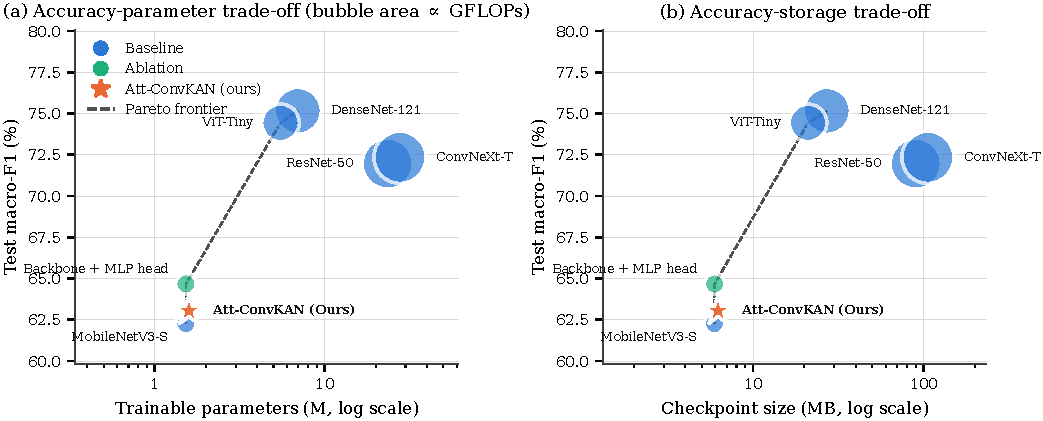
\includegraphics[width=0.74\textwidth]{fig5_pareto_efficiency.pdf}
\caption{Accuracy--efficiency trade-off on the DermaMNIST test set. Bubble area is proportional to GFLOPs; the dashed line connects Pareto-optimal models (higher macro-F1 at lower cost).}
\label{fig:pareto}
\end{figure*}

\begin{table}[!t]
\centering
\caption{Ablation study of the Att-ConvKAN components (same backbone, data, budget and seed). $\Delta$F1: macro-F1 change w.r.t.\ the backbone + MLP-head reference (row 1). Symb.: share of KAN-head edges whose spline term is $<1\%$ of their SiLU weight, i.e.\ edges that reduce to the symbolic form $w_b\,\mathrm{SiLU}(x)$; $H$: normalised entropy of the spline edge importances (lower = more concentrated).}
\label{tab:ablation}
\setlength{\tabcolsep}{2.2pt}
\resizebox{\columnwidth}{!}{%
\begin{tabular}{cccc cccc c cc c}
\toprule
\rotatebox{90}{KANConv} & \rotatebox{90}{Attention} & \rotatebox{90}{KAN head} & \rotatebox{90}{Spline reg.} & B-Acc. & Macro-F1 & AUROC & ECE$\downarrow$ & Head (K) & Symb. (\%) & $H$ & $\Delta$F1 \\
\midrule
-- & -- & -- & -- & 69.07 & 64.67 & 94.65 & 20.50 & \underline{599.2} & -- & -- & -- \\
-- & -- & \checkmark & \checkmark & 70.12 & \underline{65.57} & \textbf{95.19} & 20.00 & \textbf{374.4} & 100.0 & 0.061 & +0.90 \\
-- & \checkmark & -- & -- & \underline{70.90} & 62.87 & 94.73 & \textbf{17.73} & \underline{599.2} & -- & -- & -1.80 \\
\checkmark & \checkmark & \checkmark & -- & \textbf{71.65} & \textbf{66.23} & \underline{94.97} & \underline{19.06} & \textbf{374.4} & 41.2 & 0.858 & +1.56 \\
\midrule
\checkmark & \checkmark & \checkmark & \checkmark & 67.90 & 63.05 & 94.43 & 20.59 & \textbf{374.4} & 100.0 & 0.001 & -1.62 \\
\bottomrule
\end{tabular}}
\end{table}


\subsection{Ablation study}
Table~\ref{tab:ablation} isolates each component on the same backbone, data, budget and seed. Replacing the MLP head by the regularised KAN head (row~2) raises macro-F1 from \res{ablation_1_backbone_mlp}{macro_f1}\% to \res{ablation_2_backbone_kan_no_att}{macro_f1}\% and gives the highest AUROC of the family (\res{ablation_2_backbone_kan_no_att}{auroc}\%) with \res{derived}{head_reduction_pct}\% fewer head parameters. Adding attention to the MLP head (row~3) raises balanced accuracy (\res{ablation_3_backbone_att_mlp}{balanced_accuracy}\% vs.\ \res{ablation_1_backbone_mlp}{balanced_accuracy}\%) and lowers ECE, but not macro-F1. The full architecture without spline regularisation (row~4) obtains the highest balanced accuracy (\res{ablation_4_full_no_spline_reg}{balanced_accuracy}\%) and macro-F1 (\res{ablation_4_full_no_spline_reg}{macro_f1}\%) of the lightweight family.

The spline regulariser is the component with the clearest effect, and it is a trade-off. With $\lambda_1=1$, $\lambda_H=0.1$ the L1 and entropy terms drive almost all spline coefficients to zero: \res{att_convkan_proposed}{kan_edge_sparsity_pct}\% of the head's \res{att_convkan_proposed}{kan_head_edges_k}\,K edges reduce to the purely symbolic form $w_b\,\mathrm{SiLU}(x)$ and the normalised edge entropy falls to $H=\res{att_convkan_proposed}{kan_spline_entropy}$, versus \res{ablation_4_full_no_spline_reg}{kan_edge_sparsity_pct}\% and $H=\res{ablation_4_full_no_spline_reg}{kan_spline_entropy}$ without regularisation. The price is \res{paired@ablation_4_full_no_spline_reg}{delta_macro_f1} macro-F1 points relative to row~4 (paired 95\% CI [\res{paired@ablation_4_full_no_spline_reg}{delta_macro_f1_ci_lower}, \res{paired@ablation_4_full_no_spline_reg}{delta_macro_f1_ci_upper}], $p\res{paired@ablation_4_full_no_spline_reg}{p_value}$). Because Adam normalises each parameter's step, even a weak regularisation gradient moves an unused coefficient by roughly the learning rate per step, so the strength of the sparsity pressure is governed less by $\lambda$ than by whether an edge receives any data gradient; selecting $\lambda_1,\lambda_H$ on the validation set is therefore necessary and is left to future work. None of the differences between the full model and its ablations is significant under the paired bootstrap ($p\ge\res{derived}{min_ablation_p}$), so with a single seed and ten epochs they should be read as trends.

\begin{table}[!t]
\centering
\caption{Per-class test performance (\%) of Att-ConvKAN (Ours). Best class per column in \textbf{bold}, second \underline{underlined}.}
\label{tab:perclass}
\setlength{\tabcolsep}{3.5pt}
\begin{tabular}{l r ccccc}
\toprule
Class & $n$ & Prec. & Rec./Sens. & F1 & Spec. & AUROC \\
\midrule
\texttt{akiec} & 66 & 50.00 & 60.61 & 54.79 & 97.94 & 95.24 \\
\texttt{bcc} & 103 & 60.75 & 63.11 & 61.90 & 97.79 & 96.86 \\
\texttt{bkl} & 220 & 57.74 & 62.73 & 60.13 & 94.34 & 91.44 \\
\texttt{df} & 23 & 38.46 & 65.22 & 48.39 & \underline{98.79} & \textbf{99.03} \\
\texttt{mel} & 223 & 55.93 & 44.39 & 49.50 & 95.62 & 87.15 \\
\texttt{nv} & 1341 & \textbf{90.71} & \underline{89.56} & \textbf{90.13} & 81.48 & 93.98 \\
\texttt{vasc} & 29 & \underline{66.67} & \textbf{89.66} & \underline{76.47} & \textbf{99.34} & \underline{97.34} \\
\midrule
Macro avg. & 2005 & 60.04 & 67.90 & 63.05 & 95.04 & 94.43 \\
\bottomrule
\end{tabular}
\end{table}


\subsection{Per-class behaviour and calibration}
Table~\ref{tab:perclass} reports per-class results of \ours. The majority class \texttt{nv} reaches \res{att_convkan_proposed}{nv_f1}\% F1, and the rare vascular lesions \res{att_convkan_proposed}{vasc_recall}\% recall. Melanoma is the hardest class to detect (\res{att_convkan_proposed}{mel_recall}\% recall, \res{att_convkan_proposed}{mel_f1}\% F1); it has the lowest recall of all classes for eight of the ten models, and even \bestbaselinename\ reaches only \res{derived}{best_baseline_mel_recall}\%. Its AUROC of \res{att_convkan_proposed}{mel_auroc}\% shows that the ranking is informative but the decision threshold, shaped by the class weights, favours \texttt{nv}. Fig.~\ref{fig:roc} shows the per-class ROC and precision-recall curves and Fig.~\ref{fig:cm} the confusions, which are dominated by \texttt{mel}$\leftrightarrow$\texttt{nv}, followed by \texttt{nv}$\leftrightarrow$\texttt{bkl}.

All models are markedly \emph{under-confident} (ECE \res{att_convkan_proposed}{ece}\% for \ours), a known side effect of focal loss and class re-weighting. Temperature scaling fitted on the validation set ($T=\res{att_convkan_proposed}{temperature}$) reduces the ECE of \ours\ to \res{att_convkan_proposed}{ece_temperature_scaled}\% without changing its predictions. Split-conformal prediction sets calibrated at $\alpha=0.1$ achieve \res{att_convkan_proposed}{conformal_coverage}\% empirical coverage with \res{att_convkan_proposed}{conformal_set_size} labels per image on average, which is a practical way to flag ambiguous lesions for review.

\begin{figure*}[!t]
\centering
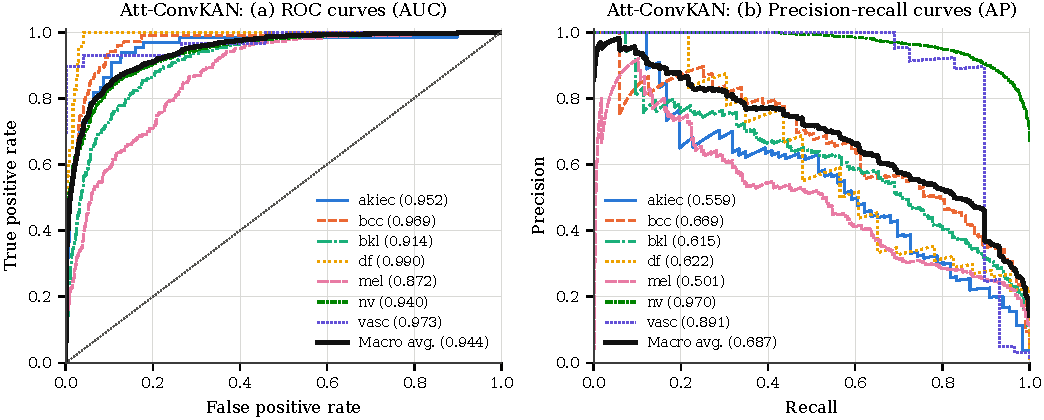
\includegraphics[width=0.66\textwidth]{fig3_roc_and_pr_curves.pdf}
\caption{Per-class and macro-average ROC (left) and precision-recall (right) curves of \ours\ on the test set; AUC and average precision in the legends.}
\label{fig:roc}
\end{figure*}

\begin{figure*}[!t]
\centering
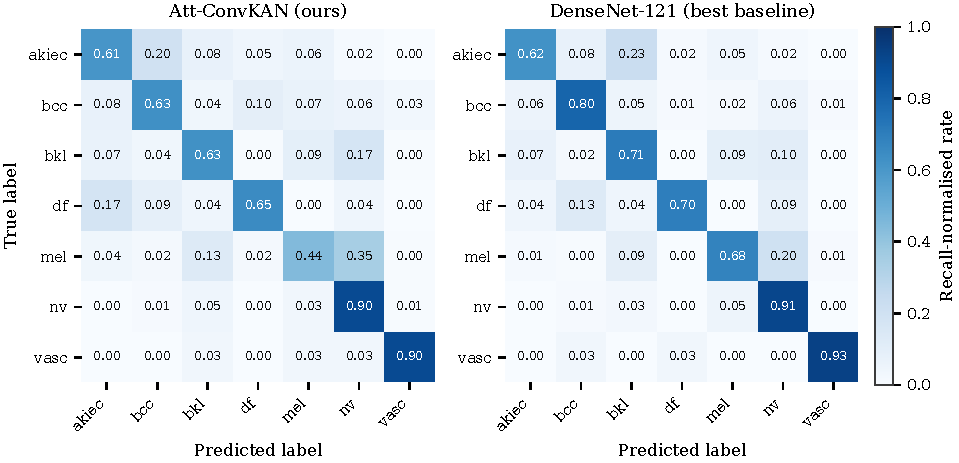
\includegraphics[width=0.56\textwidth]{fig4_confusion_matrix.pdf}
\caption{Row-normalised confusion matrices of \ours\ and the best baseline (\bestbaselinename) on the test set.}
\label{fig:cm}
\end{figure*}

\begin{figure*}[!t]
\centering
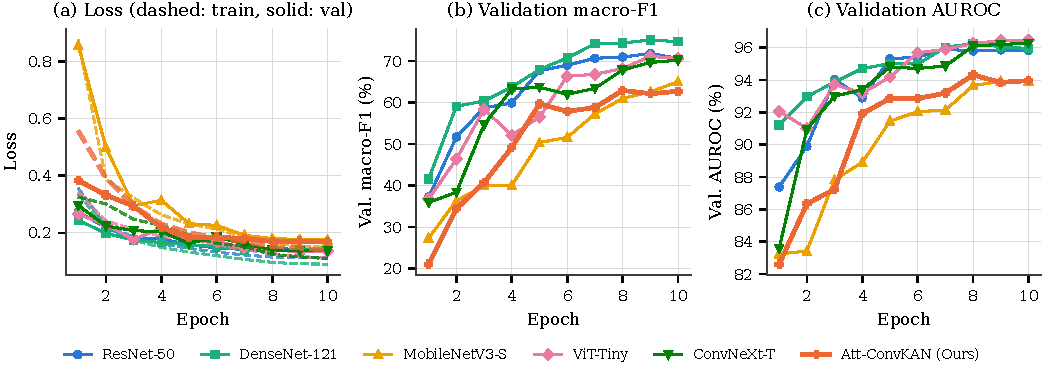
\includegraphics[width=0.7\textwidth]{fig6_training_dynamics.pdf}
\caption{Training dynamics: training (dashed) and validation (solid) loss, validation macro-F1 and validation AUROC per epoch.}
\label{fig:dynamics}
\end{figure*}

\textbf{Training dynamics.} Fig.~\ref{fig:dynamics} shows that validation macro-F1 is still rising at the end of the ten-epoch budget for most models (the best epoch of \ours\ is \res{att_convkan_proposed}{best_epoch}), so all numbers in this paper are lower bounds on what each architecture reaches with full training.

\section{Explainability Analysis}
\begin{figure*}[!t]
\centering
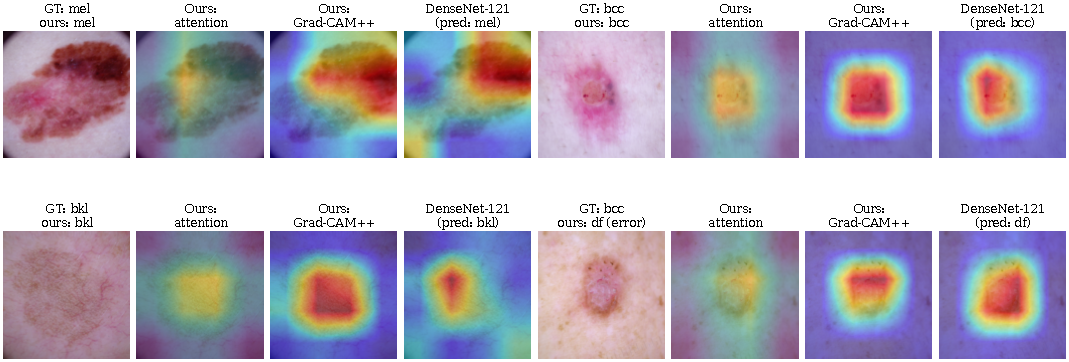
\includegraphics[width=\textwidth]{fig1_gradcam_comparison.pdf}
\caption{Qualitative explanations on four test images (three confident correct predictions of different classes and the most confident misclassified non-nevus lesion). For each image: input with ground truth (GT) and prediction of \ours; its coordinate-channel attention; its Grad-CAM++; Grad-CAM++ of the best baseline.}
\label{fig:gradcam}
\end{figure*}

\begin{figure*}[!t]
\centering
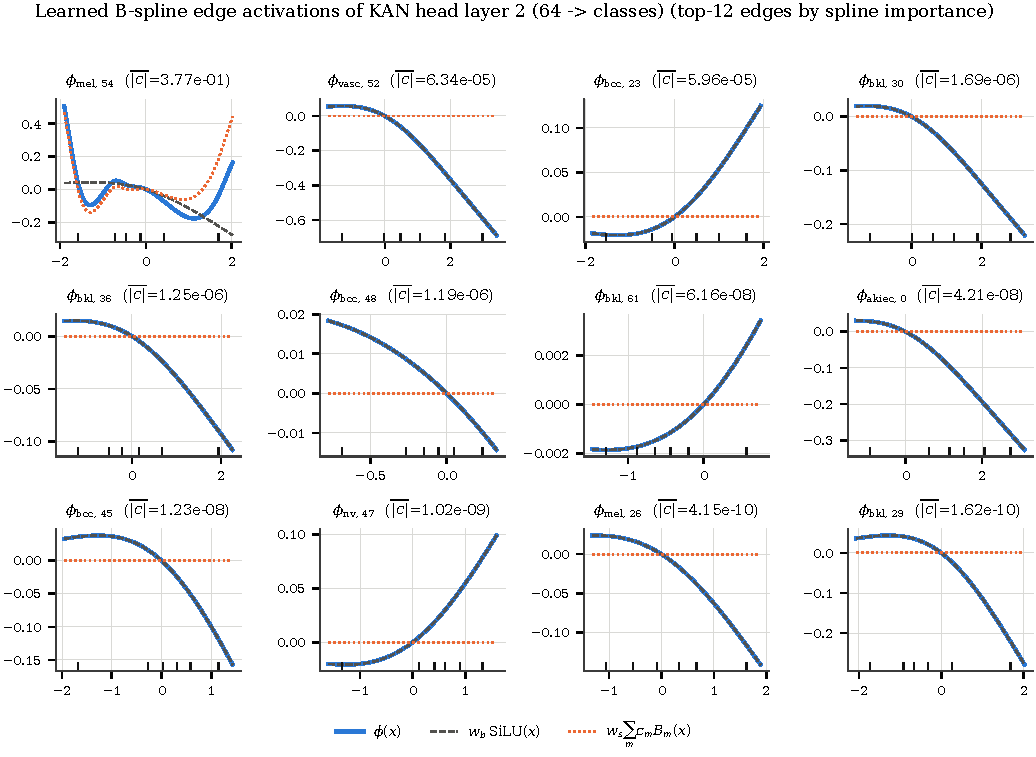
\includegraphics[width=0.6\textwidth]{fig2b_learned_kan_splines_output.pdf}
\caption{Learned edge functions $\phi_{c,i}(x)$ of the output \texttt{KANLinear} layer of \ours\ (top-12 edges by spline importance; subscripts give the target class and the input unit). Solid: total activation; dashed: SiLU residual; dotted: B-spline component; ticks: adapted knots; $\overline{|c|}$: mean absolute spline coefficient.}
\label{fig:splines}
\end{figure*}

\textbf{Spatial explanations.} Fig.~\ref{fig:gradcam} compares the attention map and Grad-CAM++ of \ours\ with Grad-CAM++ of the best baseline. At $128\times128$ input the last feature maps of both MobileNetV3 and \bestbaselinename\ are only $4\times4$, so all saliency maps are coarse. The Grad-CAM++ maps of \ours\ cover the lesion in the shown examples, and its attention masks are diffuse, acting mainly by down-weighting the image corners and borders (where vignetting and ruler artefacts occur) rather than by delineating the lesion; neither resolves lesion borders or individual dermoscopic structures. The misclassified example (a basal cell carcinoma predicted as dermatofibroma) is misclassified in the same way by \bestbaselinename, with a similarly placed saliency map. Higher input resolution (the $224\times224$ default configuration) or an earlier, higher-resolution feature level would be needed for clinically useful localisation.

\textbf{Functional explanations.} The distinctive property of a KAN is that the mapping from features to class scores can be read off directly. Fig.~\ref{fig:splines} plots the most important learned edges of the output layer. Consistent with the statistics in Table~\ref{tab:ablation}, the regularised head is almost entirely \emph{symbolic}: nearly every edge is a scaled SiLU, which can be written in closed form, and the spline capacity is concentrated on very few edges with non-monotone shapes (the top edge, feeding the melanoma logit, has two local minima). This yields a compact description of the classifier, i.e.\ a sum of SiLU terms plus a handful of tabulated univariate functions, which an MLP head cannot provide. The repository additionally plots the first head layer and the unregularised model (ablation~4), whose spline components are spread across many edges, and a per-image script (\texttt{inference\_demo.py}) that marks the actual input value on each contributing edge.

\section{Limitations}
The study uses a single seed, a ten-epoch budget, $128\times128$ inputs and CPU-only training; most models had not converged, so absolute numbers are below published DermaMNIST results at $224\times224$ and differences of a few points are within noise (paired $p>0.05$ for all ablations). The spline-regularisation weights were not tuned, and the observed collapse indicates that they should be. Latency was measured on one CPU; the relative cost of the B-spline recursion will differ on GPUs.

\section{Conclusion}
We presented \ours, a lightweight hybrid of a pretrained MobileNetV3-S backbone, a depthwise KANConv bottleneck, coordinate-channel attention and a B-spline KAN classification head, together with a pure-PyTorch KAN implementation and a fully reproducible benchmark. Under an identical short training budget on DermaMNIST, \ours\ performs on par with its MobileNetV3-S baseline (\res{att_convkan_proposed}{macro_f1}\% vs.\ \res{mobilenetv3_small}{macro_f1}\% macro-F1) while replacing a \res{mobilenetv3_small}{head_params_k}\,K-parameter MLP head by a \res{att_convkan_proposed}{head_params_k}\,K-parameter KAN head whose decision function is \res{att_convkan_proposed}{kan_edge_sparsity_pct}\% symbolic. The KAN head improved on the MLP head with fewer parameters, the full architecture without spline regularisation gave the best lightweight macro-F1, and spline regularisation traded \res{derived}{reg_cost_f1} macro-F1 points for interpretability. On CPU the spline evaluation raises single-image latency from \res{mobilenetv3_small}{latency_ms} to \res{att_convkan_proposed}{latency_ms}\,ms, so FLOP counts overstate the efficiency of KAN layers. Larger baselines, led by \bestbaselinename\ at \res{derived}{param_ratio_best_baseline}$\times$ the parameter count, remain clearly more accurate. Future work will tune the regularisation on validation data, train at full resolution and length with multiple seeds, and test whether KAN heads help on other MedMNIST tasks.



\begin{thebibliography}{99}
\footnotesize
\bibitem{esteva2017dermatologist} A.~Esteva, B.~Kuprel, R.~A. Novoa, J.~Ko, S.~M. Swetter, H.~M. Blau, and S.~Thrun, ``Dermatologist-level classification of skin cancer with deep neural networks,'' \emph{Nature}, vol.~542, no.~7639, pp.~115--118, 2017.
\bibitem{codella2019isic} N.~Codella, V.~Rotemberg, P.~Tschandl, M.~E. Celebi, S.~Dusza, D.~Gutman, B.~Helba, A.~Kalloo, K.~Liopyris, M.~Marchetti, H.~Kittler, and A.~Halpern, ``Skin lesion analysis toward melanoma detection 2018: A challenge hosted by the International Skin Imaging Collaboration (ISIC),'' \emph{arXiv:1902.03368}, 2019.
\bibitem{tschandl2018ham10000} P.~Tschandl, C.~Rosendahl, and H.~Kittler, ``The HAM10000 dataset, a large collection of multi-source dermatoscopic images of common pigmented skin lesions,'' \emph{Scientific Data}, vol.~5, art.~180161, 2018.
\bibitem{yang2023medmnist} J.~Yang, R.~Shi, D.~Wei, Z.~Liu, L.~Zhao, B.~Ke, H.~Pfister, and B.~Ni, ``MedMNIST v2 -- A large-scale lightweight benchmark for 2D and 3D biomedical image classification,'' \emph{Scientific Data}, vol.~10, art.~41, 2023.
\bibitem{liu2025kan} Z.~Liu, Y.~Wang, S.~Vaidya, F.~Ruehle, J.~Halverson, M.~Solja\v{c}i\'{c}, T.~Y. Hou, and M.~Tegmark, ``KAN: Kolmogorov-Arnold networks,'' in \emph{Proc. Int. Conf. Learn. Represent. (ICLR)}, 2025.
\bibitem{liu2024kan2} Z.~Liu, P.~Ma, Y.~Wang, W.~Matusik, and M.~Tegmark, ``KAN 2.0: Kolmogorov-Arnold networks meet science,'' \emph{arXiv:2408.10205}, 2024.
\bibitem{kolmogorov1957} A.~N. Kolmogorov, ``On the representation of continuous functions of many variables by superposition of continuous functions of one variable and addition,'' \emph{Doklady Akademii Nauk SSSR}, vol.~114, no.~5, pp.~953--956, 1957.
\bibitem{deboor1978splines} C.~de~Boor, \emph{A Practical Guide to Splines}. New York, NY, USA: Springer-Verlag, 1978.
\bibitem{bodner2024convkan} A.~D. Bodner, A.~S. Tepsich, J.~N. Spolski, and S.~Pourteau, ``Convolutional Kolmogorov-Arnold networks,'' \emph{arXiv:2406.13155}, 2024.
\bibitem{drokin2024kanconv} I.~Drokin, ``Kolmogorov-Arnold convolutions: Design principles and empirical studies,'' \emph{arXiv:2407.01092}, 2024.
\bibitem{yang2025kat} X.~Yang and X.~Wang, ``Kolmogorov-Arnold transformer,'' in \emph{Proc. Int. Conf. Learn. Represent. (ICLR)}, 2025.
\bibitem{li2025ukan} C.~Li, X.~Liu, W.~Li, C.~Wang, H.~Liu, Y.~Liu, Z.~Chen, and Y.~Yuan, ``U-KAN makes strong backbones for medical image segmentation and generation,'' in \emph{Proc. AAAI Conf. Artif. Intell.}, vol.~39, 2025, pp.~4652--4660.
\bibitem{li2024fastkan} Z.~Li, ``Kolmogorov-Arnold networks are radial basis function networks,'' \emph{arXiv:2405.06721}, 2024.
\bibitem{bozorgasl2024wavkan} Z.~Bozorgasl and H.~Chen, ``Wav-KAN: Wavelet Kolmogorov-Arnold networks,'' \emph{arXiv:2405.12832}, 2024.
\bibitem{he2016resnet} K.~He, X.~Zhang, S.~Ren, and J.~Sun, ``Deep residual learning for image recognition,'' in \emph{Proc. IEEE Conf. Comput. Vis. Pattern Recognit. (CVPR)}, 2016, pp.~770--778.
\bibitem{huang2017densenet} G.~Huang, Z.~Liu, L.~van~der~Maaten, and K.~Q. Weinberger, ``Densely connected convolutional networks,'' in \emph{Proc. IEEE Conf. Comput. Vis. Pattern Recognit. (CVPR)}, 2017, pp.~4700--4708.
\bibitem{howard2019mobilenetv3} A.~Howard, M.~Sandler, G.~Chu, L.-C. Chen, B.~Chen, M.~Tan, W.~Wang, Y.~Zhu, R.~Pang, V.~Vasudevan, Q.~V. Le, and H.~Adam, ``Searching for MobileNetV3,'' in \emph{Proc. IEEE/CVF Int. Conf. Comput. Vis. (ICCV)}, 2019, pp.~1314--1324.
\bibitem{dosovitskiy2021vit} A.~Dosovitskiy, L.~Beyer, A.~Kolesnikov, D.~Weissenborn, X.~Zhai, T.~Unterthiner, M.~Dehghani, M.~Minderer, G.~Heigold, S.~Gelly, J.~Uszkoreit, and N.~Houlsby, ``An image is worth 16x16 words: Transformers for image recognition at scale,'' in \emph{Proc. Int. Conf. Learn. Represent. (ICLR)}, 2021.
\bibitem{liu2022convnext} Z.~Liu, H.~Mao, C.-Y. Wu, C.~Feichtenhofer, T.~Darrell, and S.~Xie, ``A ConvNet for the 2020s,'' in \emph{Proc. IEEE/CVF Conf. Comput. Vis. Pattern Recognit. (CVPR)}, 2022, pp.~11976--11986.
\bibitem{hu2018senet} J.~Hu, L.~Shen, and G.~Sun, ``Squeeze-and-excitation networks,'' in \emph{Proc. IEEE/CVF Conf. Comput. Vis. Pattern Recognit. (CVPR)}, 2018, pp.~7132--7141.
\bibitem{woo2018cbam} S.~Woo, J.~Park, J.-Y. Lee, and I.~S. Kweon, ``CBAM: Convolutional block attention module,'' in \emph{Proc. Eur. Conf. Comput. Vis. (ECCV)}, 2018, pp.~3--19.
\bibitem{hou2021coordatt} Q.~Hou, D.~Zhou, and J.~Feng, ``Coordinate attention for efficient mobile network design,'' in \emph{Proc. IEEE/CVF Conf. Comput. Vis. Pattern Recognit. (CVPR)}, 2021, pp.~13713--13722.
\bibitem{lin2017focal} T.-Y. Lin, P.~Goyal, R.~Girshick, K.~He, and P.~Doll\'{a}r, ``Focal loss for dense object detection,'' in \emph{Proc. IEEE Int. Conf. Comput. Vis. (ICCV)}, 2017, pp.~2980--2988.
\bibitem{cui2019classbalanced} Y.~Cui, M.~Jia, T.-Y. Lin, Y.~Song, and S.~Belongie, ``Class-balanced loss based on effective number of samples,'' in \emph{Proc. IEEE/CVF Conf. Comput. Vis. Pattern Recognit. (CVPR)}, 2019, pp.~9268--9277.
\bibitem{selvaraju2017gradcam} R.~R. Selvaraju, M.~Cogswell, A.~Das, R.~Vedantam, D.~Parikh, and D.~Batra, ``Grad-CAM: Visual explanations from deep networks via gradient-based localization,'' in \emph{Proc. IEEE Int. Conf. Comput. Vis. (ICCV)}, 2017, pp.~618--626.
\bibitem{chattopadhay2018gradcampp} A.~Chattopadhay, A.~Sarkar, P.~Howlader, and V.~N. Balasubramanian, ``Grad-CAM++: Generalized gradient-based visual explanations for deep convolutional networks,'' in \emph{Proc. IEEE Winter Conf. Appl. Comput. Vis. (WACV)}, 2018, pp.~839--847.
\bibitem{guo2017calibration} C.~Guo, G.~Pleiss, Y.~Sun, and K.~Q. Weinberger, ``On calibration of modern neural networks,'' in \emph{Proc. Int. Conf. Mach. Learn. (ICML)}, 2017, pp.~1321--1330.
\bibitem{angelopoulos2021gentle} A.~N. Angelopoulos and S.~Bates, ``A gentle introduction to conformal prediction and distribution-free uncertainty quantification,'' \emph{arXiv:2107.07511}, 2021.
\bibitem{loshchilov2017sgdr} I.~Loshchilov and F.~Hutter, ``SGDR: Stochastic gradient descent with warm restarts,'' in \emph{Proc. Int. Conf. Learn. Represent. (ICLR)}, 2017.
\bibitem{loshchilov2019adamw} I.~Loshchilov and F.~Hutter, ``Decoupled weight decay regularization,'' in \emph{Proc. Int. Conf. Learn. Represent. (ICLR)}, 2019.
\bibitem{zhang2018mixup} H.~Zhang, M.~Cisse, Y.~N. Dauphin, and D.~Lopez-Paz, ``mixup: Beyond empirical risk minimization,'' in \emph{Proc. Int. Conf. Learn. Represent. (ICLR)}, 2018.
\bibitem{yun2019cutmix} S.~Yun, D.~Han, S.~J. Oh, S.~Chun, J.~Choe, and Y.~Yoo, ``CutMix: Regularization strategy to train strong classifiers with localizable features,'' in \emph{Proc. IEEE/CVF Int. Conf. Comput. Vis. (ICCV)}, 2019, pp.~6023--6032.
\end{thebibliography}

\end{document}
